\documentclass[nogrid]{MBE}%
\usepackage[ruled,vlined]{algorithm2e}
%\usepackage[utf8]{inputenc}
\usepackage{url}
\usepackage{parskip}
\usepackage{multicol}
\usepackage{multirow}
%\documentclass[tikz,border=10pt]{standalone}
\usepackage{tikz}
\usepackage{diagbox}
\usepackage[linguistics]{forest}
\usepackage{enumerate}
\usepackage{caption}
\usepackage{subcaption}
\usepackage{float}
\usepackage{soul}
% \usepackage{nameref}
% \usepackage{varioref}
% \usepackage{hyperref}
% \usepackage{cleveref}
\jshort{mst}

\volname{}

\jvolume{0}

\jvol{}

\jissue{0}

\pubyear{2013}

\mstype{Article}

\artid{xxx}

\access{Advance Access publication March 3, 2013}

\tikzset{
  treenode/.style = {align=center, inner sep=0pt, text centered,
    font=\sffamily},
  arn_n/.style = {treenode, circle, blue, draw=blue, text width=1.5em, very thick},% arbre rouge noir, noeud noir
  arn_r/.style = {treenode, circle, red, draw=red, text width=1.5em, very thick},% arbre rouge noir, noeud rouge
  arn_o/.style = {treenode, circle, orange, draw=orange, text width=1.5em, very thick},
  arn_x/.style = {treenode, rectangle, draw=black,
    minimum width=0.5em, minimum height=0.5em}% arbre rouge noir, nil
}

% \usepackage{multicol,lipsum,xparse}

% \let\multicolmulticols\multicols
% \let\endmulticolmulticols\endmulticols

% \RenewDocumentEnvironment{multicols}{mO{}}
%  {%
%   \ifnum#1=1
%     #2%
%   \else % More than 1 column
%     \multicolmulticols{#1}[#2]
%   \fi
%  }
%  {%
%   \ifnum#1=1
%   \else % More than 1 column
%     \endmulticolmulticols
%   \fi
%  }

\begin{document}
\captionsetup[figure]{labelfont={bf},labelformat={default},labelsep=period,name={ALG.}}

\title[Paper]{distAngsd: Novel and Fast Phylogeny Inference Methods that Allow for Uncertainties Introduced by Sequencing and Low Coverage}


\author[Zhao et al.]{{Lei} \surname{Zhao},$^{1}$  Rasmus Nielsen$^{1,2}$, and Thorfinn Sand Korneliussen,$^{1,3,*}$}

\address{$^{1}$Section for Geogenetics, Globe Institute, University of Copenhagen, Øster Voldgade 5-7, 1350 København K\\
$^{2}$Department of Integrative Biology
3040 Valley Life Sciences Building 3140 Berkeley, CA 94720-3140\\
$^{3}$National Research University, Higher School of Economics, 20 Myasnitskaya Ulitsa, 101000, Moscow, Russia}

% \history{Received 13 July 2011; reviews returned 26 November 2012; accepted 30 November 2012}

\coresp{E-mail: tskorneliussen@sund.ku.dk}
\editor{}

\datade{}


%\editor{Robb Brumfield}
%max 250 words, currently at 150.
%Format: Articles have an abstract of up to 250 words. This is followed by sections (in order) with headings: Introduction, Results, Discussion, and Materials and Methods. Results and Discussion may be combined. Subsections are allowed throughout. For articles describing new or improved methods and resources, authors should add a section entitled New Approaches after the Introduction. This section should clearly and succinctly present the new or improved methods or approaches, with extensive details provided in the Materials and Methods section, if necessary (See General Author Guidelines for all other information on manuscript preparation).
%%https://academic.oup.com/mbe/pages/Manuscript_Types

\abstract{The work presented here is focused on the inference of the divergence time between two samples in the context of low coverage next generation sequencing data. Two methods are implemented and recommended in this software suite named \textbf{distAngsd}:  distAngsd-geno and distAngsd-nuc. These novel two methods utilizes the full information of the sequencing data, by taking into account the uncertainty that  are inherent to data from this platform. We show through extensive simulations that these methods are markedly better and have more stable statistical behaviors than the all current available methods, even for very low depth data with artificially high error rates. The program is threaded, scales linearly in the number of cores allocated to the software, it is supplied as an opensource \textbf{c/c++} program under the GPL license hosted at github. Importantly it is user friendly and allows for various standard formats that will enable researches to integretate these methods and gain more inference accuracy.}

\keyword{Phylogeny reconstruction, Genotype likelihood, EM algorithm, Divergence time, maximum likelihood, highthroughput sequencing, next generation sequencing, molecular evolution, phylogenetic, genetic distance}

\maketitle

% \section{Questions For Thorfinn}
% 1. I am thinking about whether to put all the stuff together in one paper or split it into two?
% The materials we have at hand are the basic inference methods, comparisons of pre-existing methods and will include an analysis of real data.

% But based on this method, we can try to use the pairwise ML divergence times to reconstruct tree and use the whole tree structure to infer the among site rate  variation distribution. The idea of this can be found in the paper {\color{red}Phylogeny reconstruction: increasing the accuracy of
% pairwise distance estimation using Bayesian inference of
% evolutionary rates}. The results of these are not at hand now. Do you think it is too much for a paper if we combine these in one paper?

% 2. I can not say I totally understood NGSDist, and I may need you to justify the descriptions on it and results derived from its extension version later on.

% 3. I could not figure out a way to only use genotype likelihood information for ALG. \ref{algor:Nuc2SFS}, but at least your idea of using homogenous likelihood may not be right here. The way I present ALG. \ref{algor:Nuc2SFS} here is still to use the reads and their quality data. We can discuss on this later.

% 4. "distAngsd-nuc" and "distAngsd-geno" are not good enough for the methods' names, they are for temporary use. Please come up with something fancy while reading! Thanks a lot!
\vspace{2mm}
\section{{Introduction}\label{sec:Intro}}
The calculation of distance between pairs of individuals is normally the first step in the construction of a distance matrix which is then used in the construction of a phylogenetic tree. 
%The studies on genetics, archaeology, and anthropology sometimes need to deal with biological materials . Once decoded, the genetic information of such materials can help us understand the evolutionary history of humans and other species better, some information may also shed light on the studies of ecology, diseases, culture, and other relevant subjects.

Recent developments within biotechnology, specificly the advent Next Generation Sequencing (NGS or high-throuhput sequencing HTS), made it possible to get access to full genome at affordable prices. This has triggered a burst of materials and has given researchers the possibility of analysing full genomes at the population level. However the technology itself does not give direct access to the true biological variation but rather yields millions or billions of small fragment  through a massively parallel sequencing process which is essentially a sampling by replacement procedure. In a resequencing study these fragments are then stitched together or aligned relative to a haploid representation of the target genome. As an additional layer of complexity the raw DNA sequences are by themselves associated with a nonnegliable error-rate and genotype likelihoods are being calculated to capture and mitigate these errors in the genotype or consensus calling. 

With genetic analysis methods applied, the genomic data collected from modern populations of species by scientists can be used to interpret how the species were formed, what difficulties the species are now facing, and what will be the most probable destiny of the species. Thanks to the advanced preservation measures, modern genomic materials is often of good quality and accurate. Apart from the modern materials, a comparable proportion of ancient data obtained from archaeology and anthropology can also contribute to genetic studies. Such historical data from extinct species or ancient populations will serve as anchor points to unveil the detailed evolutionary events, such as mutations, selections, migrations, and demographic changes occurring between/within species or populations. Though genetically informative, ancient genomic materials suffer from badly preservation and postmortem effects, which result in lower read coverage and larger calling error rate when conducting NGS. As a consequence, more uncertainty needs to be handled when ancient DNA are being analyzed.

A family of continuous time Markov chain models of nucleotide substitution has been developed to infer the genetic divergence relationships between samples of DNA sequences. The main idea of these models is that at the molecular level, each nucleotide of the hereditary material, i.e., DNA, has a certain chance to be substituted by another nucleotide during its error-prone replications. Such substitution processes which can be modeled by continuous Markov chain, are used to measure the genetic distances among DNA sequences. Based on different assumptions of substitution rates between nucleotides, these models can be divided into three categories: JC69 \citep{Jukes_Cantor:1969} and K80 \citep{Kimura:1980} models require equal rates of substitutions between any two nucleotides; F81 \citep{Felsenstein:1981}, HKY85 \citep{Hasegawa_Kishino_Yano:1985}, F84 \citep{Felsenstein_Churchill:1996}, TN93 \citep{Tamura_Nei:1993} and more generally GTR (Generalized Time Reversible models) model \citep{Tavare:1986} are based on the assumption that the substitution rate matrix are time reversible, while the UNREST model \citep{Yang:1994} is the most general model as no extra assumption on the Markov chain has been made. Throughout this work, we will focus on the GTR model, as the probability transition matrix is diagonalizable which made it mathematically more mathematically tackleable.  

Although the models of nucleotide substitution can measure the genetic divergence relationships between DNA sequences. Phylogenomic reconstructions within species or between closely related species can still be difficult as they potentially contain a relatively high proportion of heterozygous sites (Sota and Vogler 2003). Diploid or multiploid information is not compatible in these models. Previous methods trying to handle with heterozygous sites include 1, Phasing, i.e., reconstructing haploid from diploid or multiploid samples (e.g., with PHASE \citep{Stephens_Smith_Donnelly:2001,Stephens_Donnelly:2003} or BEAGLE \citep{Browning_Browning:2007}). 2, ignoring all the heterozygous sites \citep{Maldonado_Arrabal_Rosenzvit_Oliveira_Kamenetzky:2019},  or 3, treating heterozygous as IUPAC ambiguity codes \citep{Potts_Hedderson_Grimm:2014,Schrempf_Minh_Maio_Haeseler_Kosiol:2016}. Phasing algorithms require relatively higher coverage and smaller errors, and furthermore, even with appropriate coverage and error, the lengths of short reads often limit the capacity for the algorithms to phase nucleotide bases with long physical distances \citep{Garrick_Sunnucks_Dyer:2010}. Therefore, Phasing is not a good method for phylogenomic reconstructions for badly preserved genomic materials. Ignoring all the heterozygous sites or treating heterozygous as IUPAC ambiguity codes have been known to cause biased phylogenetic estimations \citep{Lischer_Excoffier_Heckel:2014}.

{\color{red}Other methods may require for larger read depth/informative reference?}

The reconstruction of phylogenies of ancient organisms/species also confronts the problem of high uncertainties caused by low coverage and high calling error. Understanding or modelling the mechanisms of the postmortem effects and NGS technology estimates how likely a certain genotype (if the level of ploidy is known) can be the true case given the observed error-prone short reads callings at a specific site. Such estimates are called genotype likelihoods. Integrating all reads information, genetic inferences based on genotype likelihoods are more stable compared with the inferences based on incomplete reads information (e.g., inferences based on a randomly chosen read per site or the consensus calling). To our best knowledge, NGSDist \citep{Vieira_Lassalle_Korneliussen_Fumagalli:2015} is the only pre-existing method using the information of genotype likelihood to infer the genetic distances between diploid individuals. As NGSDist is not based on a clear molecular evolution model, it may estimate the relative relatedness, but genetic distance inferred cannot directly tell the divergence time between different individuals/genetic samples.

Two novel divergence time concatenated inference methods, distAngsd-geno and distAngsd-nuc, are present in this work. Based on the GTR model of nucleotide substitution, both of the methods are pairwise ML estimators. Making use of the genotype likelihoods, distAngsd-geno is designed for analyzing the known diploid samples (and can be extended to any known multiploid samples) of bad quality (especially, ancient samples with low coverage and high calling error). And distAngsd-nuc requires no information about the ploidy level. Taking uncertainties of all reads into account, the method of distAngsd-nuc can be used to estimate the divergence time of samples with unknown ploidy or the samples with different ploidy. The basic idea of both methods is similar: 1, Use the EM algorithm to estimate the joint distribution of genotypes (distAngsd-geno) or the joint distribution of sampled nucleotides for both samples (distAngsd-nuc). 2, Such joint distributions then serve as pseudo-observations when calculate the likelihood functions of the GTR model. 3, Maximize the likelihood to infer the divergence time between samples. 

Simulations are conducted for comparisons among the presented methods and some of the pre-existing inference methods. The inferred results of the recommended methods have fewer biases and smaller variances especially when the read depth is lower, or the variable genome length is shorter. Different methods are also applied to the published data. The inferred phylogenetic trees based on the recommended methods match better the prior species knowledge than those based on pre-existing methods according to a topological measurement.

\vspace{2mm}
\section{Models and Methods}\label{sec:ModelsandMethods}
Both distAngsd-geno and distAngsd-nuc share similar characteristics: Firstly an estimate of the joint distribution of either genotypes (distAngsd-geno) or sampled nucleotides (distAngsd-nuc) is obtained based on either genotype likelihood data or the observed reads and their quality scores. Such joint distributions can then be interpretated as \emp{pseudo-observations} and serve as a basis for inferring the actual distance measure using the classic  maximum likelihood approaches from molecular evolutionary models, e.g., the JC69 model or the more general GTR model.

\vspace{2mm}
\subsection{EM Estimation of joint distributions}\label{subsec:EM}
As a relatively low read depth and high calling error rate are assumed, it is not sufficient to use the short reads information for a single nucleotide base to obtain a meaningful nucleotide/genotype inference. Statistic inference has to conducted across all the informative sites (When the site has read depths $\geq 1$ for both samples, we count it as an informative site). In order to make inference of genetic distance between samples, the joint distribution of genotypes (distAngsd-geno) or the joint distribution of sampled nucleotides for both samples (distAngsd-nuc) per site will be estimated given the observed short reads data. The inferred joint distributions will play a role as pseudo-observations when the JC69 or GTR model likelihood function is evaluated. The joint distributions will be inferred via EM algorithm \citep{Dempster_Laird_Rubin:1977}:

In distAngsd-geno, the joint genotype distribution can be presented in a 10 by 10 matrix $\bf M$. $10$ is the total number of all possible genotypes of a diploid individual at per site, i.e., {AA, AC, AG, AT, CC, CG, CT, GG, GT, TT}. Both row and column of $\bf M$ are indexed by these genotypes. And every element of $\bf M$, ${\bf M}(g_i,g_j)$, represents the proportion of the informative sites where the true genotypes of the focal pair of samples are given by its row and column, i.e., $g_i$ and $g_j$ correspondly.

While in distAngsd-nuc, a 4 by 4 matrix $\bf N$ representing the joint distribution of sampled nucleotides per site is estimated. $4$ is the number of all possible sampled nucleotides, i.e., {A, C, G, T}. Each row or column of $\bf N$ is indexed by one of these nucleotides. And every element in $\bf{N}$, ${\bf N}(n_i,n_j)$, denotes the proportion of the true sampled read pairs $(n_i,n_j)$ per informative site.

\begin{figure}
\begin{algorithm*}[H]\label{algor:Geno2SFS}
\SetAlgoLined
\SetKw{KwBy}{by}
% \KwResult{Write here the result }
\Comment{{\bf Input:} Genotype likelihoods of sites}\;
\Comment{{\bf Output:} $10\times 10$ matrix $\bf{M}$}\;
 initialization: ${\bf M}_{0}(g_i,g_j)\gets\frac{1}{100}$, $t\gets 0$\;
 \While{elements in $\bf{M}$ do not converge}{
 ${\bf M}_{t+1}(g_i,g_j)\gets 0$\;
 \For{$s\gets1$ \KwTo $\#sites$}{
    \If{$s$ is an informative site}{
    \vspace{2mm}
    ${\bf M}_{t+1}(g_i,g_j)\gets {\bf M}_{t+1}(g_i,g_j)+\frac{{\bf M}_{t}(g_i,g_j)\mathrm{GL}_1(s,g_i)\mathrm{GL}_2(s,g_j)}{\sum\limit_{g_i,g_j}{\bf M}_{t}(g_i,g_j)\mathrm{GL}_1(s,g_i)\mathrm{GL}_2(s,g_j)}$\;
    }
    }
    ${\bf M}_{t+1}(g_i,g_j)\gets\frac{{\bf M}_{t+1}(g_i,g_j)}{\#\textit{informative sites}}$\;
    $t\gets t+1$\;
 }
\caption{EM estimation for $\bf{M}$}
\end{algorithm*}
\caption{EM algoritm for the $10\times10$ pesudo-observation joint genotype distribution matrix $\bf{M}$, where the notation ${\bf M}_{t}$ represents the $t$th iterative result of the matrix $\bf{M}$ and the function $\mathrm{GL}_k(s,g_i)$ is the genotype likelihood of the genotype $g_i$ at site $s$ in sample $k$.}
\end{figure}

\begin{figure}
\begin{algorithm*}[H]\label{algor:Nuc2SFS}
\SetAlgoLined
\Comment{{\bf Input:} Reads data and their quality scores}\;
\Comment{{\bf Output:} $4\times 4$ matrix $\bf N$}\;
initialization: ${\bf N}_{0}(n_i,n_j)\gets\frac{1}{16}$, $t\gets 0$\;
 \While{elements in $\bf N$ do not converge}{
  ${\bf N}_{t}(n_i,n_j)\gets 0$\;
  \For{$s\gets 1$ \KwTo $\#sites$}{
  \For{$r_1\gets 1$ \KwTo $\#reads_{s,1}$}{
  \For{$r_2\gets 1$ \KwTo $\#reads_{s,2}$}{
  \vspace{2mm}
\hspace{-2mm}${\bf N}_{t+1}(n_i,n_j)\gets {\bf N}_{t+1}(n_i,n_j)$\\
\hspace{-2mm}$+\frac{{\bf N}_{t}(n_i,n_j)P_1(s,r_1,n_i)P_2(s,r_2,n_j)}{\sum\limits_{n_i,n_j}{\bf N}_{t}(n_i,n_j)P_1(s,r_1,n_i)P_2(s,r_2,n_j)}$\;
  }
  }
  }
  ${\bf N}_{t+1}(n_i,n_j)\gets \frac{{\bf N}_{t+1}(n_i,n_j)}{\sum\limits_{s=1}^{\#\textit{sites}}\#reads_{s,1}\times\#reads_{s,2}}$\;
  $t\gets t+1$\;
 }
 \caption{\small EM estimation for matrix $\bf N$}
\end{algorithm*}
\caption{EM algoritm for the $4\times 4$ pesudo-observation joint copied nucleotide distribution matrix $\bf N$, where the notation ${\bf N}_{t}$ represents the $t$th iterative result of the matrix $\bf N$, and the function $P_l(s,r_k,n_i)$ is the likelihood function of the copied nucleotide $n_i$ of the read $r_k$ at site $s$ in sample $l$, which can be obtained from the read quality data.}
\end{figure}

distAngsd-geno infers $\bf M$ via ALG. \ref{algor:Geno2SFS}, while distAngsd-nuc applies ALG. \ref{algor:Nuc2SFS} to estimating $\bf N$. One should note that both of the EM algorithms described here are independent with the evolutionary models' adoption (e.g. JC69 model or GTR model) and can be pre-calculated. The input of ALG. \ref{algor:Geno2SFS} is the genotype likelihood data of all informative sites which can be calculated by VCFtools \cite{Danecek:2011} or GATK \cite{Poplin:2017} and present in the .vcf files. While the input in ALG. \ref{algor:Nuc2SFS} is the likelihood of sampled nucletides per read per site. This type of data can be achieved from .bam or .sam files which are the output of the DNA alignment software (e.g., BWA, \citet{Li:2013}).

\vspace{2mm}
\subsection{Maximum Likelihood Inference}\label{subsec:ML}
The EM inferred joint distribution matrices $\hat{\bf M}$ and $\hat{\bf N}$ will serve as pseudo-observations in this section when the log-likelihood function of genetic distance $d$ based on the adopted molecular evolutionary model is formulated. Maximum likelihood will be conducted to estimate the genetic distance $d$ and other related parameters.
\vspace{1mm}
\subsubsection{Log-likelihood of distAngsd-geno inference}
The log-likelihood function of distAngsd-geno given the inferred pseudo-observation matrix $\hat{\bf M}$ is as follows,
\begin{align}\label{eqn:Geno2dloglike}
 & l(d|{\bf\hat{M}}) \nonumber\\
 = &\sum_{g_1,g_2}{\bf \hat{M}}(g_1,g_2)\left\{\sum_{i,j=1}^2\log\left[\pi_{g_{1,i}}\mathrm{P}_{g_{1,i},g_{2,j}}(d)\right]\right\},
\end{align}
where $g_{1,i}$ and $g_{2,j}$ are the $i$'th and $j$'th nucleotides of genotypes $g_1$ and $g_2$ ($i,j=1$ or $2$), correspondingly. The order of the nucleotides within a genotype is fixed but regardless of phasing. In practice, we always assume that the nucleotides in a genotype follows the order A, C, G and T. For instance, both genotypes AC and CA at a site in sample $1$ will be denoted as $g_1=\mathrm{AC}$ (and hence in this case $g_{1,1}=\mathrm{A}$ and $g_{1,2}=\mathrm{C}$) $\mathrm{P}_{g_{1,i},g_{2,j}}(d)$ is the transition probability from nucleotide $g_{1,i}$ to $g_{2,j}$ given the genetic distance between the two samples is $d$. $\pi_{g_{1,i}}$ is the stationary distribution of nucleotide $g_{1,i}$.
\vspace{1mm}
\subsubsection{Log-likelihood of distAngsd-nuc inference}
The log-likelihood function of distAngsd-nuc given the inferred pseudo-observation matrix $\hat{\bf{N}}$ is,
\begin{align}\label{eqn:Nuc2dloglike}
 \hspace{-2.5mm}l(d|{\bf\hat{N}}) = \sum_{n_1,n_2}{\bf\hat{N} }(n_1,n_2)\log\left[\pi_{n_1}\mathrm{P}_{n_1,n_2}(d)\right],
\end{align}
where $\mathrm{P}_{n_1,n_2}(d)$ is the transition probability from nucleotide $n_1$ to $n_2$ given the genetic distance between the two samples is $d$. $\pi_{n_1}$ is the stationary distribution of nucleotide $n_1$. 

The forms of $\mathrm{P}_{\cdot,\cdot}(\cdot)$, $\pi_{\cdot}$ and $d$ in both Equations (\ref{eqn:Geno2dloglike}) and (\ref{eqn:Nuc2dloglike}) will be determined by the adopted substitution model (e.g., JC69 or GTR model). The pairwise genetic distance $d$ can be viewed as a compound function of divergence time $t=t_0+t_1+t_2$ (as shown in FIG. \ref{fig:basictree4inference}) between two samples and the substitution rate. If the substitution rate is assumed to be unchanged, and after some rescaling of substitution rate matrix (see Supplementary Information for details), we will have the mean number of substitutions occurring per base per scaled time unit is $1$, so $d$ and $t$ will have the identical value and the inferred $d$ can be compared with the $t$ in simulation codes (See ALG. \ref{algor:Simulation}).

In principle, given the adopted evolutionary model and the observations of a pair of samples, one can also infer more parameters in addition to the genetic distance $d$, e.g., the fraction of invariable sites $p_{inv}$. In the Supplementory Information (Section S3.5), we show that for the asymmetric evolutionary models (e.g., GTR+I), the parameters $d$ and $p_{inv}$ can be jointly estimated with acceptable variances/biases by using distAngsd-geno and distAngsd-nuc even if the genome length is as short as $100kbp$, while the other compared methods will give highly biased estimations. Though in practice, $p_{inv}$ and other phylogeny paramters are recommened to infer with more samples and in a tree structure, the accurate estimation of joint inference of $d$ and $p_{inv}$ reflects the stability of both of our methods.

\vspace{2mm}
\subsection{Simulation and Comparison}\label{subsec:SimandComp}
\vspace{1mm}
\subsubsection{Simulation}
% \begin{forest}
%   [
%     [A
%      [\textit{i}
%      ]
%      [\textit{j}
%      ]
%     ]
%     [B
%       [\textit{k}]
%       [\textit{l}]
%     ]
%   ]
% \end{forest}
% \begin{tikzpicture}[->,>=stealth',level/.style={sibling distance = 3cm/#1,
%   level distance = 1.5cm}]
\setcounter{figure}{0}
\captionsetup[figure]{labelfont={bf},labelformat={default},labelsep=period,name={FIG.}}
\begin{figure}[ht]
\begin{center}
\begin{tikzpicture}
    % place nodes
    \node[orange] at (-0.4,-0.1) {$t_1$};
    \draw [black](-0.1,1) -- (-0.3,1);
    \draw [black](-0.1,-1.2) -- (-0.3,-1.2);
    \draw [stealth-stealth,orange,ultra thick,dashed](-0.2,-1.2) -- (-0.2,1);
    \node[draw] at (1, 1)  (l1) [arn_r] {A};
    \node[draw] at (0.5,-1)  (l10) [arn_o] {i};
    \node[draw] at (1.5,-1)  (l11) [arn_o] {j};
    %child{ node [arn_n] {j}} 
    \draw[bend left,-,ultra thick, orange]  (l10) .. controls (1,1.1) .. (l11);
   
    \node[blue] at (5.5,0.2) {$t_2$};
    \draw [black](5.1,1) -- (5.3,1);
    \draw [black](5.1,-0.6) -- (5.3,-0.6);
    \draw [stealth-stealth,blue,ultra thick,dashed](5.2,-0.6) -- (5.2,1);
    \node[draw] at (4,1)  (l2) [arn_r] {B};
    \node[draw] at (3.5,-0.5)  (l20) [arn_n] {k};
    \node[draw] at (4.5,-0.5)  (l21) [arn_n] {l};
    \draw[bend left,-,ultra thick, blue]  (l20) .. controls (4,1.005) .. (l21);
    \draw[bend left,-,ultra thick, red]  (l1) .. controls (2.5,3) .. (l2);
    \draw[bend left,-,ultra thick, red, to-to,dashed]  (-0.2,1) .. controls (2.5,4.0) .. (5.2,1);
    \node[red] at (2.5,3.6) {$t_0$};
    % \node[draw] at (0, -6)  (c2)    {C};
    % \node[draw] at (5, -6)  (d2)    {D};

    % draw edges  
    % \draw[] (a2.east)   -- (b2) node[at start, above right] {$x(kT)$};
    % \draw[] (c2.east)   -- (d2) node[at start, above right] {$y(kT)$};
\end{tikzpicture}
\end{center}
\vspace{0.5cm}
\caption{Simulated divergence tree: this is the tree structure we used for simulation. Two remoting two diploid individuals are of the genotypes $ij$ and $kl$ correspondingly. The most recent common ancestor of $i$ and $j$ is A, and that of $k$ and $l$ is B. The divergence time of A and B is denoted as $t_0$, while the time from $A$ to $i$ or $j$ is $t_1$ and the time from $B$ to $k$ or $l$ is $t_2$. And we also define $t = t_0+t_1+t_2$, the divergence time between the two diploid individuals.}
\label{fig:basictree4inference}
\end{figure}
Simulations are conducted according to the ALG. \ref{algor:Simulation}. We assume that the simulated organism is diploid, which is the requirement for distAngsd-geno, and the inference of distAngsd-nuc, though more general, is also based on these simulations. The simulated phylogeny is as FIG. \ref{fig:basictree4inference}. The genotype likelihood model in simulation is the GATK genotype likelihood model (\citet{Poplin:2017} and Section S1 in Supplementary Information), which is based on the following equations,
\begin{align*}
\mathrm{P}(r_k=l|g=ij) = \left\{\begin{array}{ll}
     1-e_k, & {\rm If\hspace{0.1cm}} l=i=j,  \\
     \frac{e_k}{3}, & {\rm If\hspace{0.1cm}} l\neq i {\hspace{0.1cm}\rm and\hspace{0.1cm}} l\neq j, \\
     \frac{1}{2}-\frac{e_k}{3}, &  {\rm Otherwise,}
\end{array}\right.
\end{align*}
where $i$, $j$ and $l$ are nucleotides, and $e_k$ is the calling error rate of the $k$'th read at the focal nucleotide site. $\mathrm{P}(r_k=l|g=ij)$ represents the probability of the $k$'th read is $l$ given the true genotype is $ij$ at the focal base. 

In the simulations, It is assumed that the base calling error rates are identical across different reads and sites, which guarantees that the raw read depth and effect base depth (EBD, \citet{Wang:2013}) per site are not very much different from each other. The raw read depths of different sites are assumed to be i.id Poisson random variables in the simulations.
\setcounter{figure}{2}
\captionsetup[figure]{labelfont={bf},labelformat={default},labelsep=period,name={ALG.}}
\begin{figure}
\begin{algorithm*}[H]\label{algor:Simulation}
\SetAlgoLined
\vspace{2mm}
\Comment{{\bf Input:} Substitution rate matrix $\bf R$ (so the stationary distribution of $\pi_{\cdot}$ is known), divergence time $t$, $t_1$ and $t_2$}, calling error rate $e$, mean of read depth $\mathrm{RD}$, variable genome length $l$\;
\Comment{{\bf Output:} Reads data and Genotype likelihoods across the sites}\;
{\bf Ancestral sequences construction:} \newline
The ancestral nucleotide sequences $a_1$ and $a_2$ of two samples are simulated given $\bf R$, $\pi_{\cdot}$, divergence time $t-t_1-t_2$, and $l$, sites are assumed to evolve independently\;
{\bf Sequences construction and calling:}\newline
initialization: $\mathrm{GL}_1(s,g)\gets \mathrm{GL}_2(s,g) \gets 0$\;
\For{$j\gets 1$ \KwTo $2$}{
\vspace{2mm}
Two sequences $q_{j1}$ and $q_{j2}$ of sample $j$ are derived from $a_j$ given $\bf R$, $l$, and time $t_j$ from the ancestral sequence\;
\For{every site $s$ {\bf in} sample $j$}{
\vspace{2mm}
Generate read depth $n \sim {\bf Poisson}(\mathrm{RD})$;\newline
$n$ reads are equally attributed to the site $s$ in $q_{j1}$ and $q_{j2}$ for copying with an error rate $e$, and the observed reads are $\{r_k\}_{k=1}^n$\;
$\mathrm{GL}_j(s,g) +=\sum_{k=1}^n\log\left[{\bf Prob}(r_k|g)\right]$\;
}
}
 \caption{Simulation Scheme}
\end{algorithm*}
\caption{Simulation scheme of two individual samples with a shared ancestor, which is used to validate our inference methods. The variable genome length is the number of sites which purely satisfy the adopted molecular evolutionary model. The simulation scheme considering both variable sites and invariable sites can be found in ALG. S1 in Supplementary Information.}
\end{figure}
\vspace{1mm}
\subsubsection{Comparisons with the pre-existing methods}
Based on the same simulation scheme (ALG. \ref{algor:Simulation}), four pre-existing inference methods, i.e., RandomSEQ, ConsensusSEQ, ConsensusGT, and NGSDist are compared with the proposed methods (i.e., distAngsd-geno and distAngsd-nuc). RandomSEQ refers to the method that one read is randomly chosen per site to infer the genetic distance between individuals. ConsensusSEQ denotes the method that the consensus read (based either on physical read depth or effective base depth \citet{Wang:2013}) per site is used to infer the genetic distance between individuals. And ConsensusGT represents the method that the consensus genotype per site is used to infer the genetic distance between individuals. The consensus genotype at each site is determined by the posterior distribution of genotype given by the site's genotype likelihood. When the consensus genotype is a heterozygote, ambiguous inference methods which will be described below, is applied. 

In both RandomSEQ and ConsensusSEQ, either randomly drawn or consciously chosen reads across informative sites will be used to estimate the genetic distance. The corresponding likelihood function of both methods can be given as,
\begin{align*}
l(d|\hat{\mathbf{C}}_1)=\sum_{n_1,n_2}\hat{\mathbf{C}}_1(n_1,n_2)\log\left[\pi_{n_1}\mathrm{P}_{n_1,n_2}(d)\right],
\end{align*}
where $\hat{\mathbf{C}}_1$ is the joint drawn/chosen reads counts matrix of the size $4\times 4$ according to RandomSEQ and ConsensusSEQ. And the definitions of $\mathrm{P}_{n_1,n_2}(d)$ and $\pi_{n_1}$ are the same as those in Equation \ref{eqn:Nuc2dloglike}.

ConsensusGT takes further advantage of the prior knowledge of ploidy level. And in the context of this work, ploidy level is diploid. But phylogeny inference can not handle heterozygous sites quite well, so some works just discarded all the heterozygous sites, while others used the method of ambiguous inference, which meant to deal with the putative heterozygous sites. The heterozygous sites in the ambiguous inference method will be replaced by their corresponding IUPAC ambiguity code. For example, the site C/T will be denoted by the letter Y, which represents the pyrimidine. And the likelihood of pseudo-observations of joint genotype counts matrix $\hat{\bf C}$ is given as follows (Details of derivation, See Supplementary Material S5.1),
\begin{equation}
\hspace{-1mm}l(d|\hat{\mathbf{C}}_2) = \sum_{g_1,g_2} \hat{\mathbf{C}}_2(g_1,g_2)\left\{\log\left[\mathrm{P}_{g_1,g_2}(d)\right]\right\},\label{eqn:AmbiguousInference}
\end{equation}
where $\hat{\mathbf{C}}_2$ is the joint genotypes counts matrix of the size $10\times 10$ according to ConsensusGT.
$\log\left[\mathrm{P}_{g_1=ij,g_2=kl}(d)\right]$ has the form of $\log\left[\sum\limits_{n_1\in\{i,j\}}\pi_{n_1}\sum\limits_{n_2=\{k,l\}}\mathrm{P}_{n_1,n_2}(d)\right]$ plus a constant. If the nucleotides $i$ and $j$ of the genotype $ij$ are the same, the set $\{i,j\}$ has only $1$ element. 

When the genotypes $ij$ and $kl$ are both homogeneous, the form $\log\left[\mathrm{P}_{g_1=ij,g_2=kl}(d)\right]$ in Equation \ref{eqn:AmbiguousInference} is equivalent to the form $\sum_{i,j=1}^2\log\left[\pi_{g_{1,i}}\mathrm{P}_{g_{1,i},g_{2,j}}(d)\right]$ in Equation \ref{eqn:Geno2dloglike}. While if either the genotype $ij$ or $kl$ is heterozygous, the likelihood in Equation \ref{eqn:AmbiguousInference} will underestimate the genetic distance between samples: As in FIG. \ref{fig:basictree4inference}, the ambiguous inference likelihood tries to approximate the distance between the internal nodes A and B rather than the distance between actual genotypes of two samples, $ij$ and $kl$. If substitution rate is assumed to be so small that the times from A or B to tips are not sufficient to trigger less than $\frac{1}{2}$ substitution on average, one can view the the distribution of nucleotides at A as half the chance $i$, and half the chance $j$, and similarly the nucleotide distribution at node B can be viewed as half the chance $k$ and half the chance $l$. The genetic distance $d$ will be underestimated since it ignores the distance generated by $t_1$ and $t_2$ in FIG. \ref{fig:basictree4inference}. However, when the substitution rate or the the times from A or B to tips are large, the distributions of nucleotides at A and B can not be approximated as described above, but in general the genetic distance $d$ will be underestimated if the fraction of heterozygous sites can not be ignored and ambiguous inference is applied.

{\color{red} 

We also compare the novel methods with NGSDist \cite{Vieira_Lassalle_Korneliussen_Fumagalli:2015}, which is the only pre-existing method that make use of the genotype likelihoods to infer the genetic distances. We apply the NGSDist inference in different parameter settings, based on simulation scheme ALG. \ref{algor:Simulation}. The simulated $10$ genotype likelihoods per individual per site will be converted into major-minor-allele $3$ genotype likelihoods via Angsd \cite{Korneliussen:2014}, and the $3$ genotype likelihoods will serve as the input of NGSDist to calculate the pairwise distances.

} 

As we discussed in the Table S3 of the Supplementary Information, four pieces of information will contribute to inferring the phylogeny, i.e., the read depth, the base calling errors of each read, the nucleotide frequencies at the site and the ploidy level of the focal organism. The first three pre-existing methods (i.e., RandomSEQ, ConsensusSEQ and ConsensusGT) make only partially/no use of the base calling errors of each site and other information, while distAngsd-geno and NGSDist use all the information, and distAngsd-nuc uses all the information except ploidy level. {\color{red}However, the genetic distance defined in NGSDist (i.e.,the first two equations in \citealp{Vieira_Lassalle_Korneliussen_Fumagalli:2015}) is molecular evolutionary model free and based on the infinite site model, so 1) No recurrent mutation is allowed, which will lead to underestimations of the genetic distances defined by molecular evolutionary models; 2) Only symmetric substitution model can be inferred, which will limit the usage of NGSDist} Hence in principle, the proposed distAngsd methods should outperform all the $4$ pre-existing methods discussed above. And the results shall be presented in the Results Section.

% \begin{itemize}
% \item Infer the divergence time based on a randomly chosen read per site per individual sample. As shown in the Result section, based on maximum likelihood, if the correct model is chosen, the mean inferred divergence time should be unbiased. However, since incomplete read data is used, a larger estimator variance will be obtained compared with distAngsd-geno or distAngsd-nuc, when a sufficient poisson read depth ($\sim 0.75\times$) or a relative calling error is presented.
% \item Make inference of the divergence time via treating heterozygous sites as IUPAC ambiguity codes. By doing this, the inferences meant to take advantage of ploidy information of the data. The putative heterozygous sites will be replaced by their corresponding IUPAC ambiguity code. For instance, the site C/T will be substituted by the letter Y, which represents the pyrimidine. We combine this idea with the genotype likelihood. The corresponding likelihood function can be expressed as follows (Details of derivation, See Supplementary Material):
% \begin{equation}
% \hspace{-1mm}l(d) = \sum_{g_1,g_2}{\bf \hat{M}}(g_1,g_2)\left\{\log\left[\mathrm{P}(g_1,g_2,d)\right]\right\},\label{eqn:AmbiguousInference}
% \end{equation}
% where 
% $\log\left[\mathrm{P}(g_1=\overline{ij},g_2=\overline{kl},d)\right]$ has the form of $\log\left[\sum\limits_{n_1\in\{i,j\}}\pi_{n_1}\sum\limits_{n_2=\{k,l\}}\mathrm{P}_{n_1,n_2}(d)\right]$. If the nucleotides $i$ and $j$ of the genotype $\overline{ij}$ are the same, the set $\{i,j\}$ has only $1$ element.

% It is based on a wrong model: As in FIG. \ref{fig:basictree4inference}, it tries to infer the the divergence time between the internal nodes A and B rather than the of the tips. The form of $\mathrm{P}(\overline{ij},\overline{kl},d)$ above can be viewed as an approximation of joint distribution of nucleotides at nodes A and B:??? If substitution rate is so small that the times from A or B to tips are not sufficient to trigger less than $\frac{1}{2}$ substitution on average, one can view the the distribution of nucleotides at A as half the chance $i$, and half the chance $j$, and similarly the nucleotide distribution at node B can be viewed as half the chance $k$ and half the chance $l$. The genetic distance $d$ will be underestimated if Equation \ref{eqn:AmbiguousInference} is applied since it ignores the distance generated by $t_1$ and $t_2$ in FIG. \ref{fig:basictree4inference}. However, when the substitution rate or the the times from A or B to tips are large, the distributions of nucleotides at A and B can not be approximated as described above, but in general the genetic distance $d$ will be underestimated.

% \item {\color{red}An extended NGSDist inference method is also used to compare with the presented methods. The original NGSDist is designed only for diallelic sites in \citet{Vieira_Lassalle_Korneliussen_Fumagalli:2015}}. 
% \end{itemize}
{\color{red}
\vspace{2mm}

\iffalse
The data is aligned to a collapsed version of reference genome (v0.5, \citet{Sork:2016}; available from \url{https://valleyoak.ucla.edu/genomicre sources/}) via BWA-MEM v.0.7.17 \cite{Li:2013}. VCFtools v.0.1.17 \cite{Danecek:2011} is then applied to calculate the genotype likelihoods and get the .vcf files. The bed file of sites passing the filtering criteria in \cite{Fitz-Gibbon_Hipp_Pham_Manos_Sork:2017} of each sample is kindly shared by Dr. Fitz-Gibbon and Prof. Sork to gurantee that we are on the right track to conduct phylogeny inference. Their filtering criteria and adjustments in are as follows,
\begin{enumerate}[i]
    \item Identification of targeted genome regions and variant discovery were done with GATK v3.6-0-g89b7209 \cite{McKenna:2010}, as follows. We ran CallableLoci on each sample with default parameters, except that minimum read depth is set to 5 and maximum read depth is set to 100 (minDepth 5 and maxDepth 100). An overall set of callable regions, hereafter referred to as reference-mapped loci, included all regions of exactly 86 bp determined to be callable in at least four samples. HaplotypeCaller variant discovery is run using emitRefConfidence GVCF mode separately for each sample. The whole cohort is concurrently genotyped over the reference-mapped loci regions using GenotypeGVCFs with a minimum confidence of 30.
    \item Based on inspection of variant calls and read alignments \cite{Robinson:2011}, we chose to only filter the variants by QD as well as requiring them to be biallelic. VariantFiltration is used to apply a QD $< 2.0$ filter tag. 
    \item VCFtools v0.1.15 \cite{Danecek:2011} is used to filter non-biallelic variants. 
    \item Sites with filtered variants, including non-biallelic variants are converted to Ns for all samples (these sites are filtered out later by the phylogenic analysis software).
    \item For each sample, GATK loci not considered callable by the above CallableLoci step are converted to Ns.
    \item Sequences are printed with passing variants applied according to homozygous genotype or if heterozygous IUPAC ambiguity codes are used.
    \item Homozygous indel variants are included using dashes to maintain the overall alignment. However, there is no IUPAC ambiguity code for heterozygous indels and so they are instead encoded as Ns.
\end{enumerate}
Apart from the filtering and adjustments described above, The bed files of sites they sent to us also go through an extra round of filtering to remove the loci with more than five heterozygous sites, but as they pointed out later that "the extra filters had little effect on phylogeny topology or congruence although the relative positions of the Q. lobata and Q. engelmannii clades are altered, but with zero bootstrap support".
The filters described above had largely suppressed the fraction of heterozygous sites in the downstream phylogeny analyses, and the remaining heterozygous sites will be treated as IUPAC ambiguity codes due to the limitations of the pre-existing methods. In order to recover more heterozygous sites (non-biallelic sites) and uncertainties (low quality sites) which distAngsd-geno is believed to handle, we only used the information of positions of loci in each bed file. And for the marked Ns within the loci regions which has mapped reads information, we restored them. For every pair of oak samples, the parallel-computatinal distAngsd-geno inference with simplest JC69 model is conducted and only the sites with non-zero read depths for both samples will be used to estimate the pairwise genetic distances.  Once the $83\times 83$ pairwise matrix is determined, program PhyD \cite{Criscuolo:2008} will use the BioNJ \cite{Gascuel:1997} algorithm to build neighbour joining trees, and trees are plotted with FigTree v1.4.4. (\url{http://tree. bio.ed.ac.uk/software/figtree/}). 
\fi

\subsection{Experimental data analyses}\label{subsec:ExperimentalData}
The proposed distAngsd-geno method is applied to infer the phylogeny of the published oak dataset \cite{Fitz-Gibbon_Hipp_Pham_Manos_Sork:2017}. This RADseq dataset is comprised of $83$ oak samples representing $16$ taxa around the US. We obtained access to the raw fastq sequences and followed the reference mapped approach described in details in \citealp{Fitz-Gibbon_Hipp_Pham_Manos_Sork:2017}. {\color{blue} The sites for downstream analyses are based on the callable loci bedfiles kindly shared by Prof. Victoria L. Sork and Dr. Sorel Fitz-Gibbon through personal correspondences. For each site, we use the raw genotype likelihood for our novel approach.} 
\iffalse
\st{Our dataprocessing deviated from their pipeline by allowing heterozygote sites which was then either encoded as IUPAC ambiguity codes when comparing with existing distance methods or simply using the raw genotype likelihood for our novel approach.} 
\fi
For every pair of oak samples, the parallel-computational distAngsd-geno inference with simplest JC69 model is conducted and only the sites with non-zero read depths for both samples will be used to estimate the pairwise genetic distances.  Once the $83\times 83$ pairwise matrix is determined, program PhyD \cite{Criscuolo:2008} will use the BioNJ \cite{Gascuel:1997} algorithm to build neighbour joining trees, and trees are plotted with FigTree v1.4.4. (\url{http://tree. bio.ed.ac.uk/software/figtree/}). 

As distAngsd-geno is currently implemented for pairwise genetic distance inference and the simplest JC69 model is used for the inference of the real data, it is not very suitable to directly compare the distAngsd-geno's results with the results in the original paper \cite{Fitz-Gibbon_Hipp_Pham_Manos_Sork:2017} where they conducted such inferences based on ML tree with more complicated model, we thus compared our inference results with pre-existing methods based sorely on JC69 model, i.e., ConsensusSEQ and ConsensusGT. Bcftools consensus is applied to getting the consensus nucleotide sequence and the consensus genotype sequence of each sample. And the putative heterozygous sites in ConsensusGT are expressed as IUPAC codes. Then the pairwise distances between samples are calculated as the genetic distance 
between their consensus sequences based on the JC69 model. The neighbour joining trees are then contructed in the same way as the distAngsd-geno tree described in the previous paragraph via PhyD and FigTree v1.4.4.

Downsampling is conducted to each of the $83$ samples via samtools view -s command to further test the distAngsd-geno's inference capability when lower depth is observed. The original $83$ samples have an average read depth $20.32$ and lowest depth $10.34$. Each sample is downsampled to read depth $10$, $5$, $1$, $0.75$, $0.5$, and $0.25$ according to its original read depth. And similarly as above, phylogenetic trees will be constructed based on each downsampled set of data.}

\vspace{2mm}
\section{Results}\label{sec:Results}
In this section, both simulated and experimental results are presented to validate the proposed methods.

\vspace{2mm}
\subsection{Inferences based on simulations}\label{subsec:SimInfer}
The simulations are conducted as described in the previous section. We fix the $t_1 = 0.4$, and $t_2 = 0.25$ in FIG. \ref{fig:basictree4inference}, but vary the ancestral divergence time $t_0$, such that $t = t_0+t_1+t_2= 0.8$, $1.0$ and $1.6$. The inference results of our methods distAngsd-geno, distAngsd-nuc, as well as those of other pre-existing methods (RandomSEQ and ConsensusSEQ) are plotted in FIG. \ref{fig:JC1Mb} and FIG. \ref{fig:GTR1Mb} in the main text, FIG. S8 and FIG. S9 in the Supplementary Information.  Different figures correpond to different average read depth per site ($20$, $10$, $5$, $1$, $0.75$ or $0.5$) and different variable genome length (1Mb in the main text or 0.1Mb in the supplementary Information). Here the variable genome length is the number of sites which purely satisfy the adopted molecular evolutionary model. Base calling error is set to be $0.2\%$. Both the JC69 model and a more generalized GTR model (Table 1.3 in \citet{Yang:2006}) are applied.
  
% \begin{multicols}{1}
\setcounter{figure}{1}
\captionsetup[figure]{labelfont={bf},labelformat={default},labelsep=period,name={FIG.}}
\begin{figure*}[ht]
    \centering
    \begin{subfigure}[b]{0.475\textwidth}
         \centering
         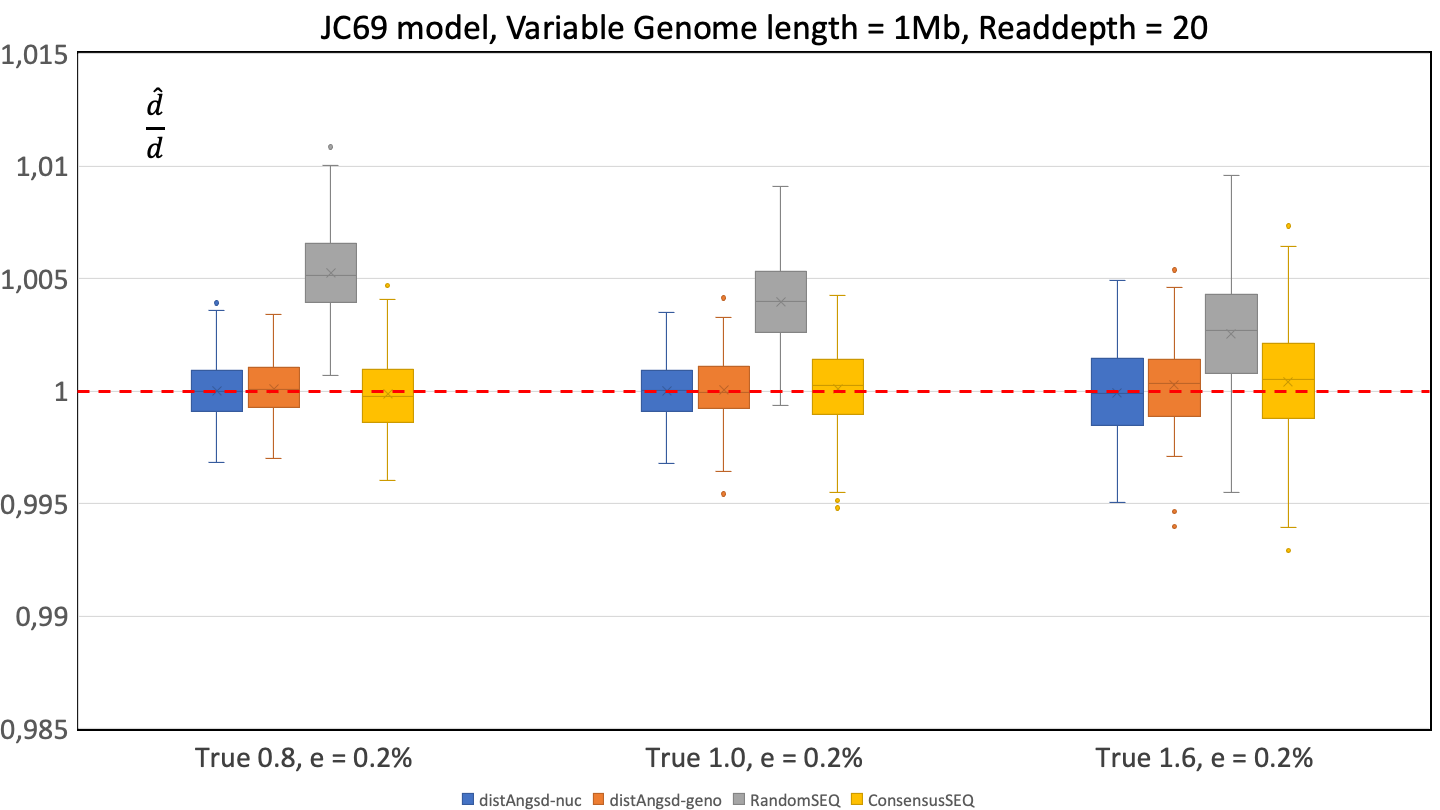
\includegraphics[width=\textwidth]{JCRD20_1Mb.png}
         \caption{}
         \label{fig:JCRD20_1Mb}
     \end{subfigure}
     \begin{subfigure}[b]{0.475\textwidth}
         \centering
         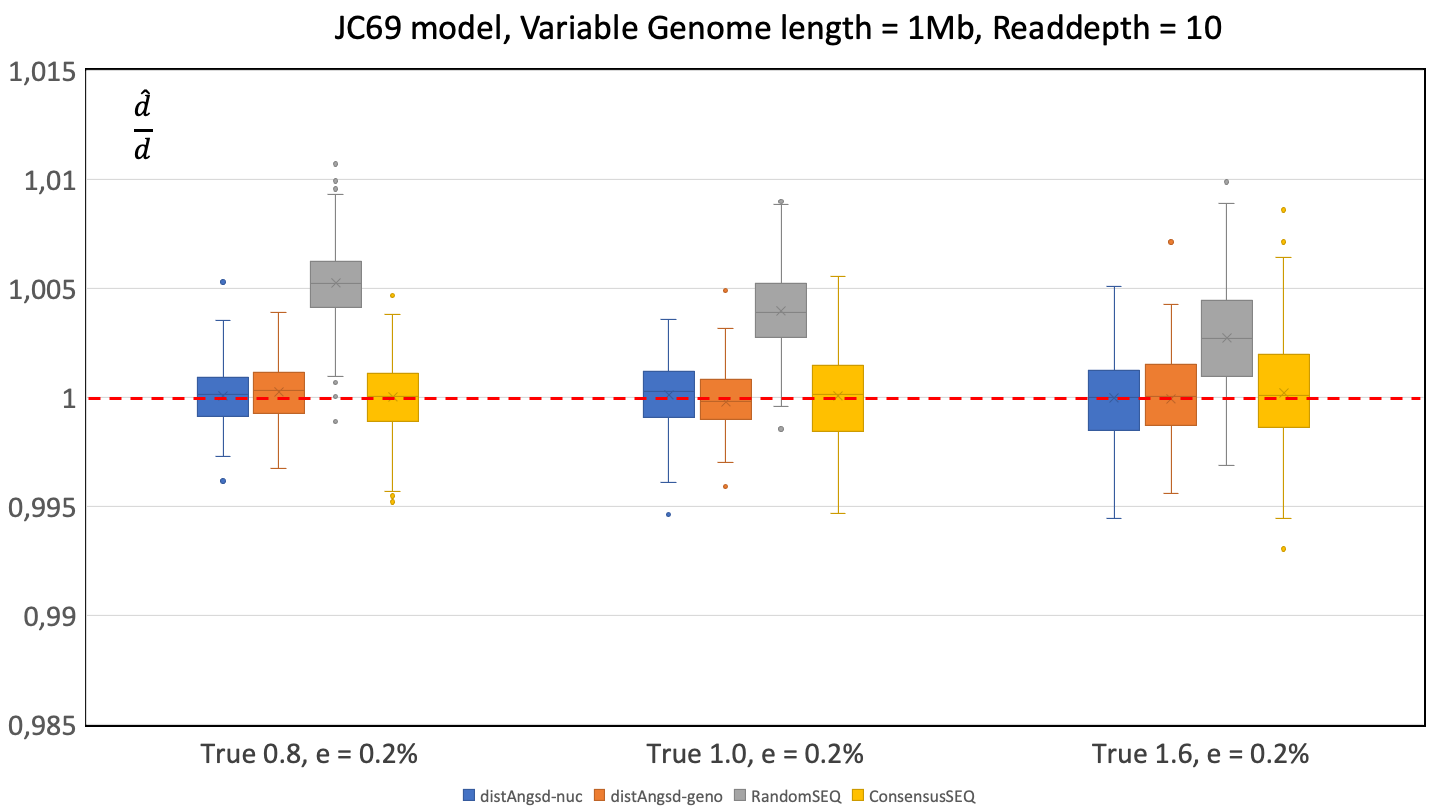
\includegraphics[width=\textwidth]{JCRD10_1Mb.png}
         \caption{}
         \label{fig:JCRD10_1Mb}
     \end{subfigure}
     \begin{subfigure}[b]{0.475\textwidth}
         \centering
         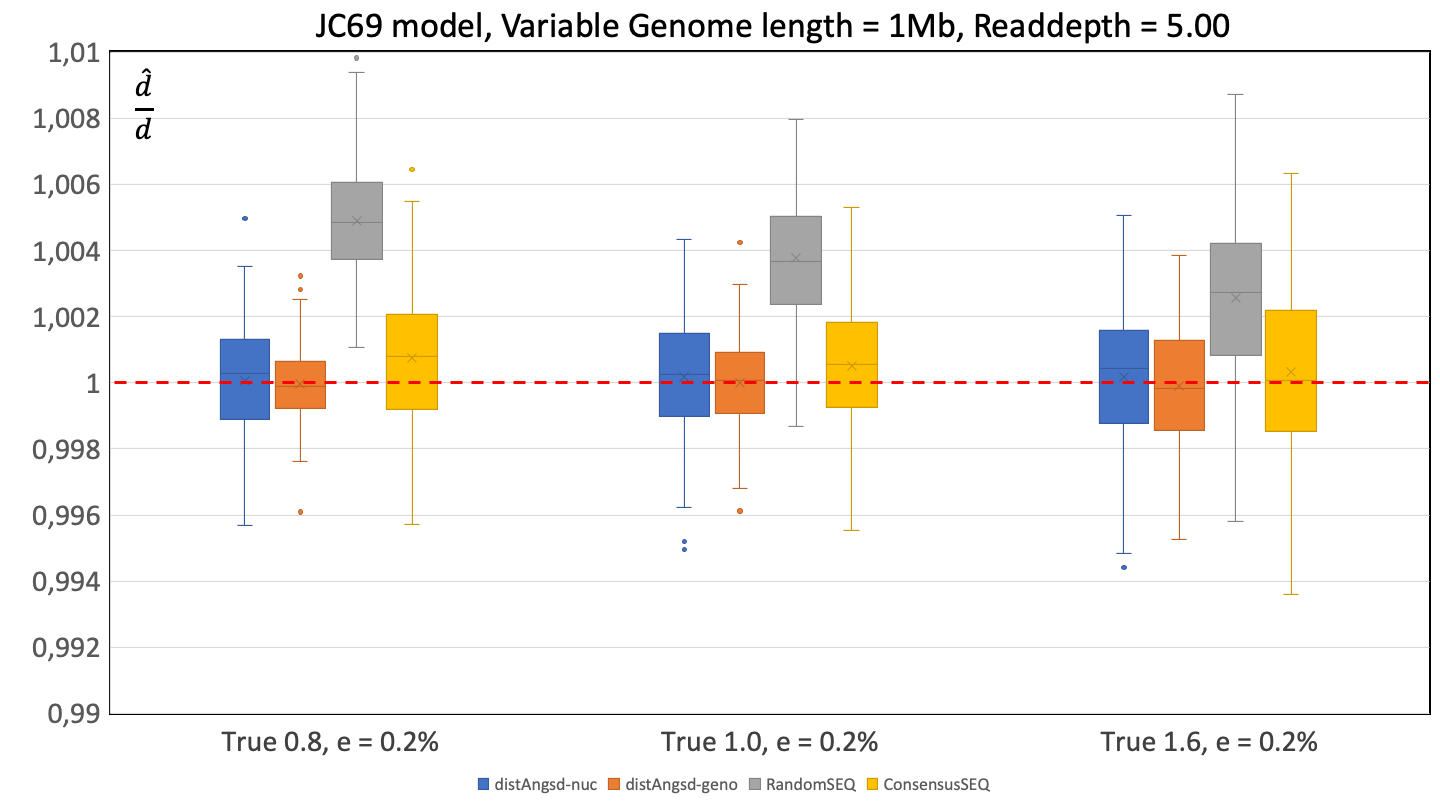
\includegraphics[width=\textwidth]{JCRD5_1Mb.png}
         \caption{}
         \label{fig:JCRD5_1Mb}
     \end{subfigure}
     \begin{subfigure}[b]{0.475\textwidth}
         \centering
         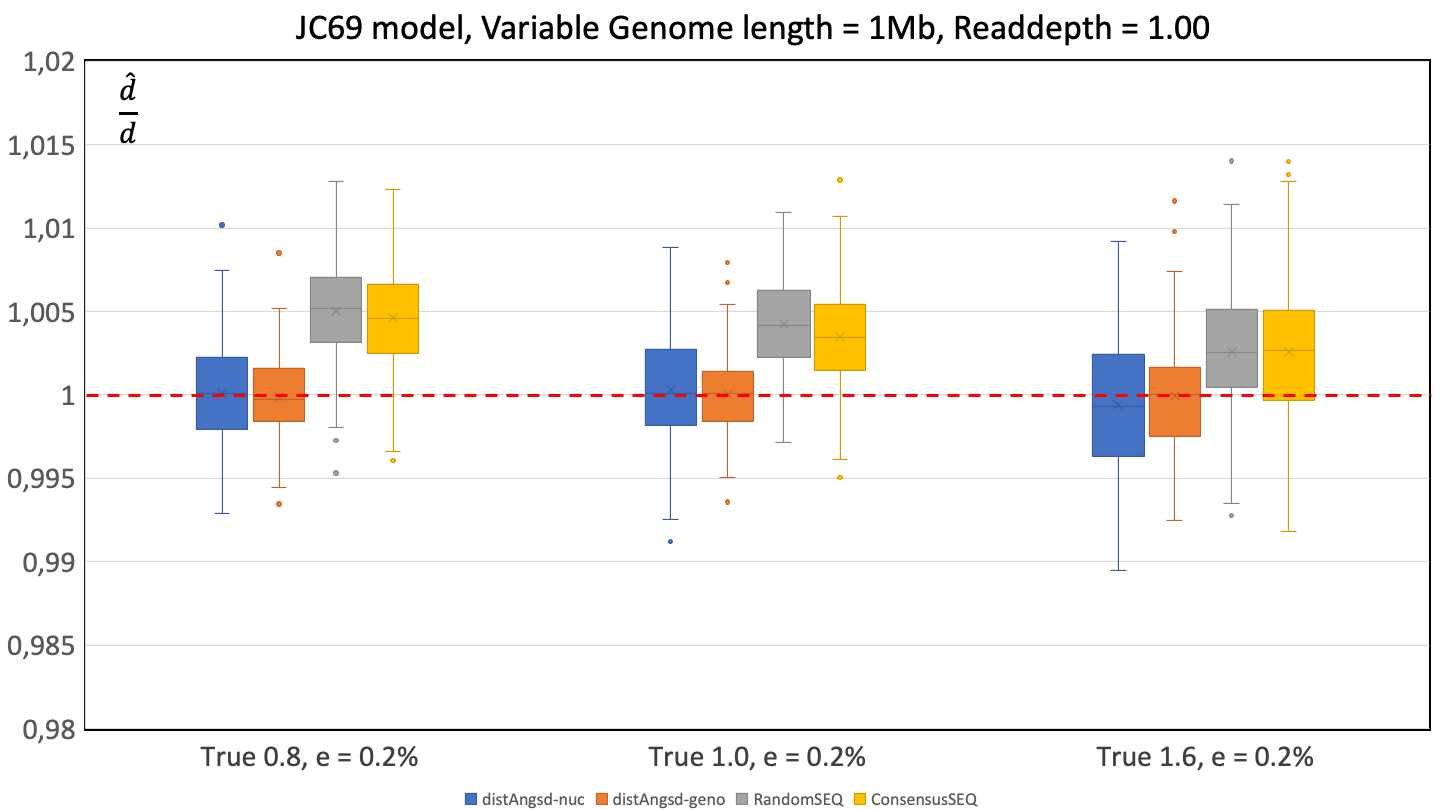
\includegraphics[width=\textwidth]{JCRD1_1Mb.png}
         \caption{}
         \label{fig:JCRD1_1Mb}
     \end{subfigure}
     \begin{subfigure}[b]{0.475\textwidth}
         \centering
         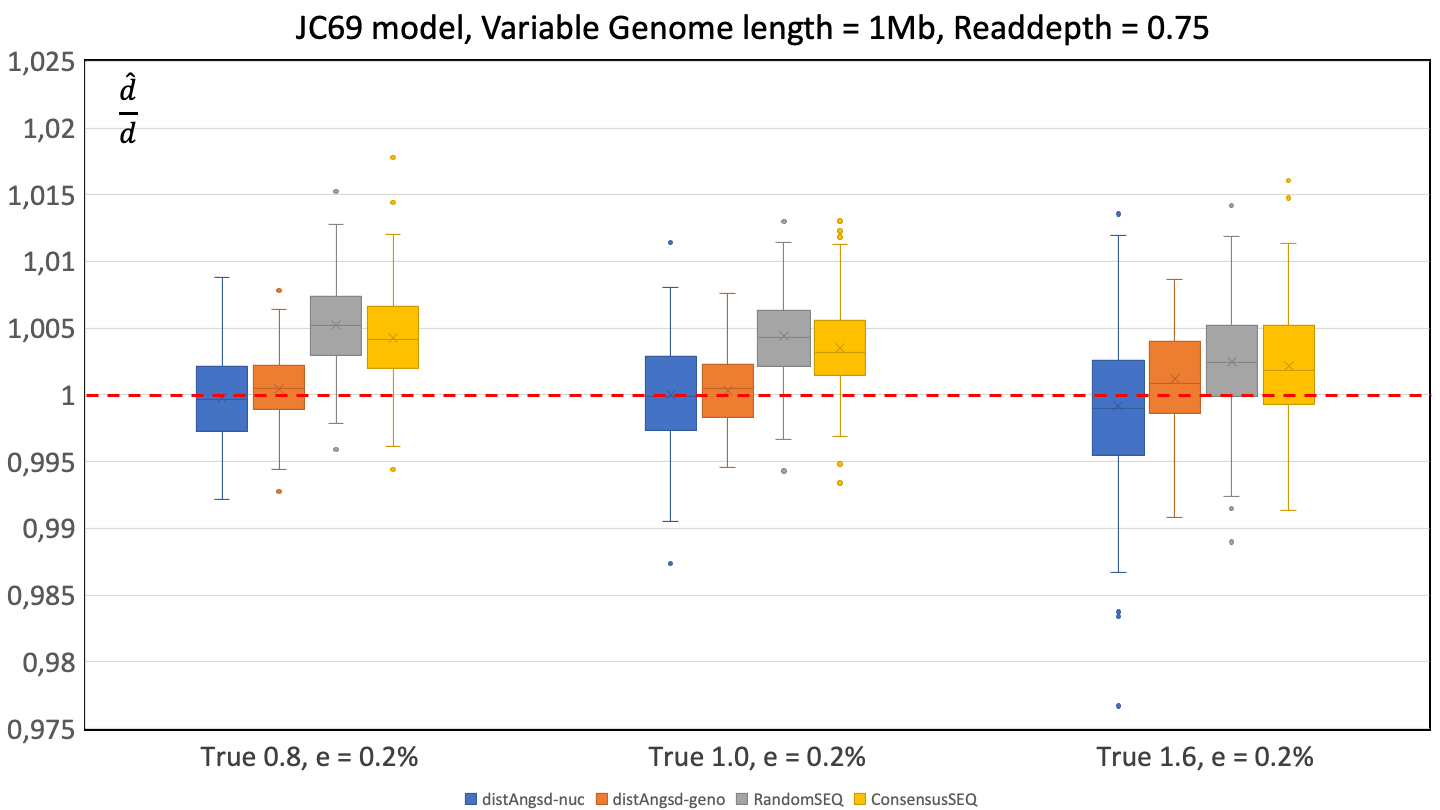
\includegraphics[width=\textwidth]{JCRD075_1Mb.png}
         \caption{}
         \label{fig:JCRD075_1Mb}
    \end{subfigure}
     \begin{subfigure}[b]{0.475\textwidth}
         \centering
         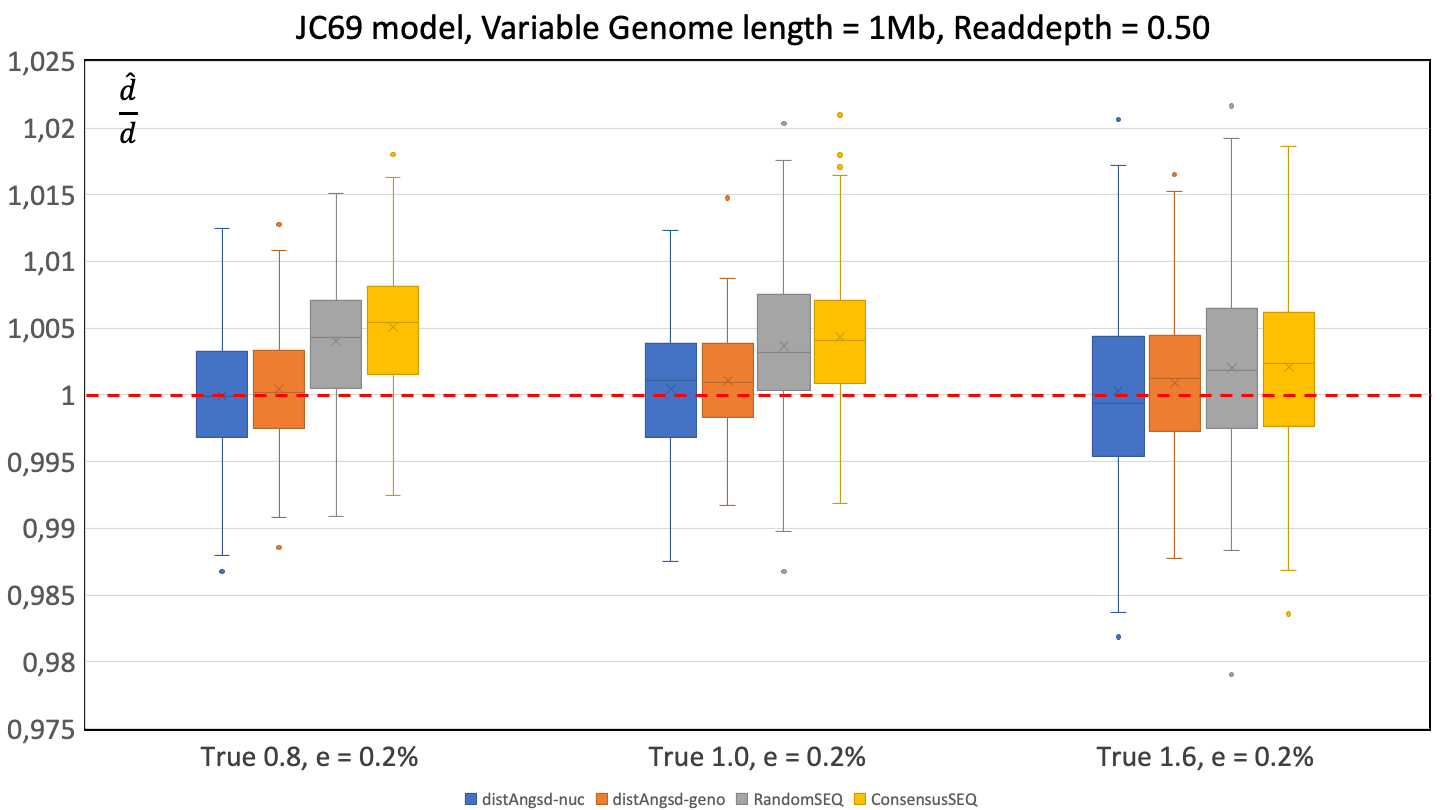
\includegraphics[width=\textwidth]{JCRD05_1Mb.png}
         \caption{}
         \label{fig:JCRD05_1Mb}
    \end{subfigure}
    % 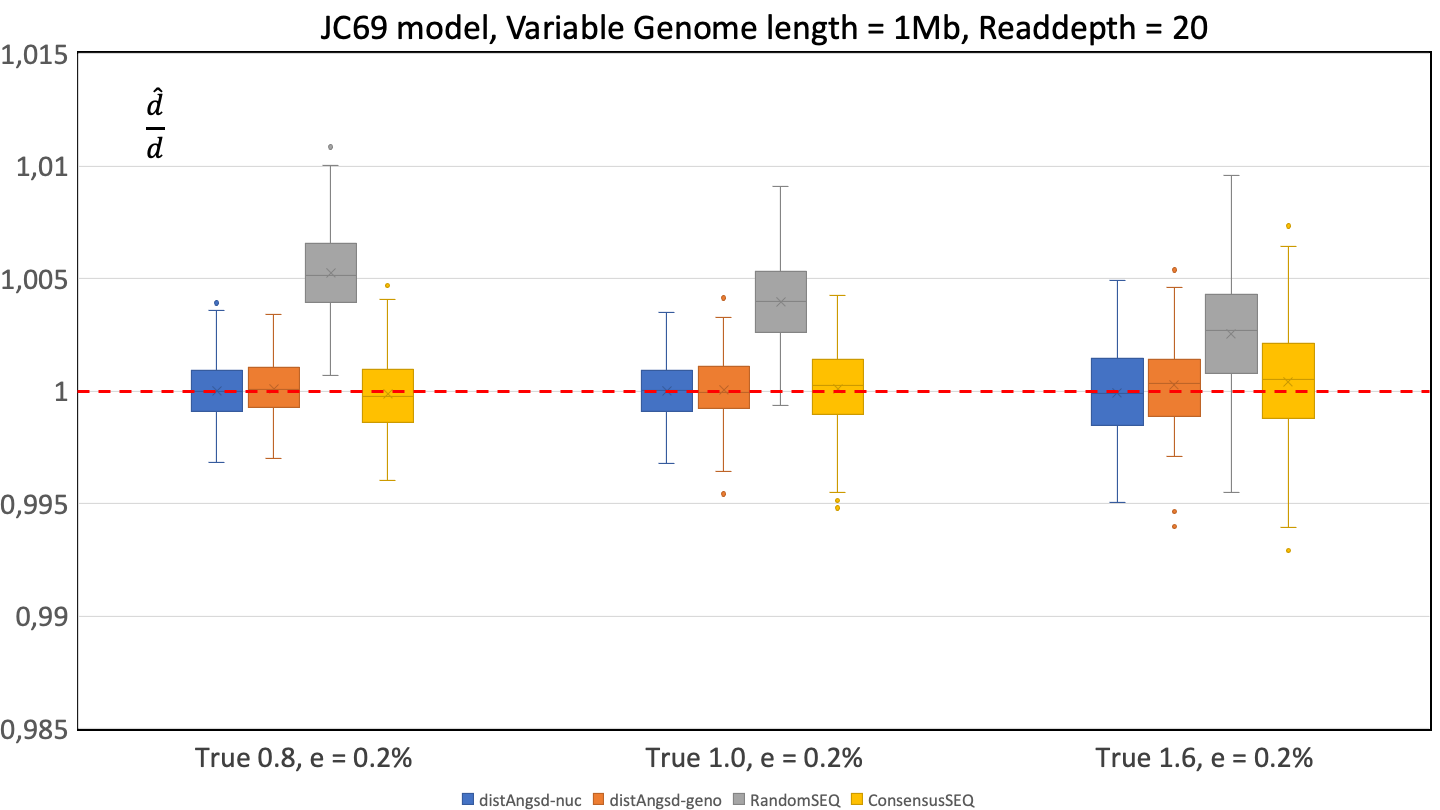
\includegraphics[width=1.9\columnwidth]{JCRD20_1Mb.png}
    \vspace{0.5cm}
    \caption{The inferred results of four different methods based $200$ replicates of JC69 model simulation, i.e., distAngsd-nuc, distAngsd-geno, RandomSEQ, and ConsensusSEQ when genome length is $1$Mb, and the average read depth per site varies from (a) $20$ to (f) $0.5$. The simulated base calling error is $e =0.2\%$. Simulated divergence tree follows Fig. \ref{fig:basictree4inference}, with $t_1=0.4$ and $t_2 = 0.25$, and true simulated divergence time $t$ (hence the genetic distance $d$) is set as $0.8$, $1.0$ and $1.6$.}
    \label{fig:JC1Mb}
\end{figure*}
% \end{multicols}
\begin{figure*}[ht]
    \centering
    \begin{subfigure}[b]{0.475\textwidth}
         \centering
         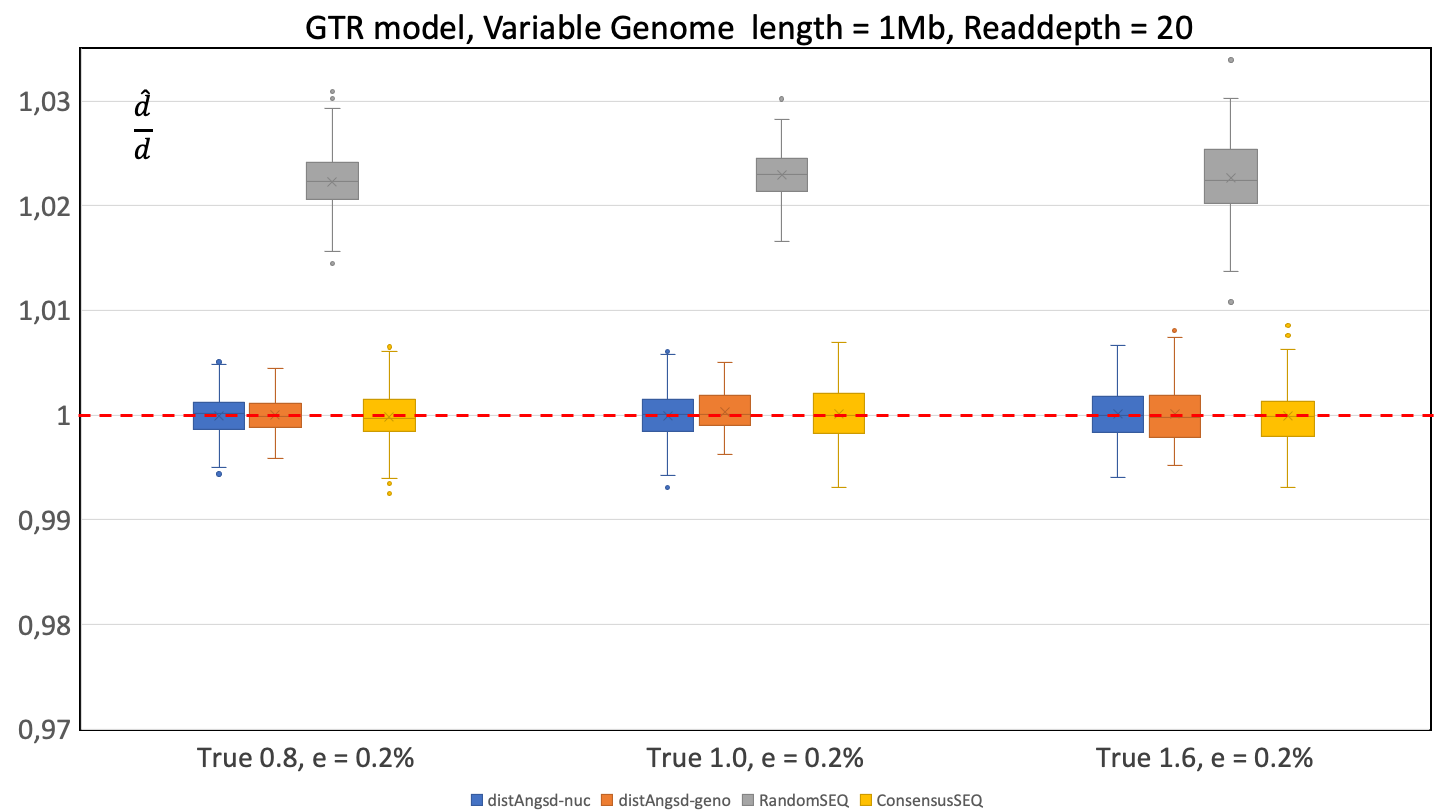
\includegraphics[width=\textwidth]{GTRRD20_1Mb.png}
         \caption{}
         \label{fig:GTRRD20_1Mb}
     \end{subfigure}
     \begin{subfigure}[b]{0.475\textwidth}
         \centering
         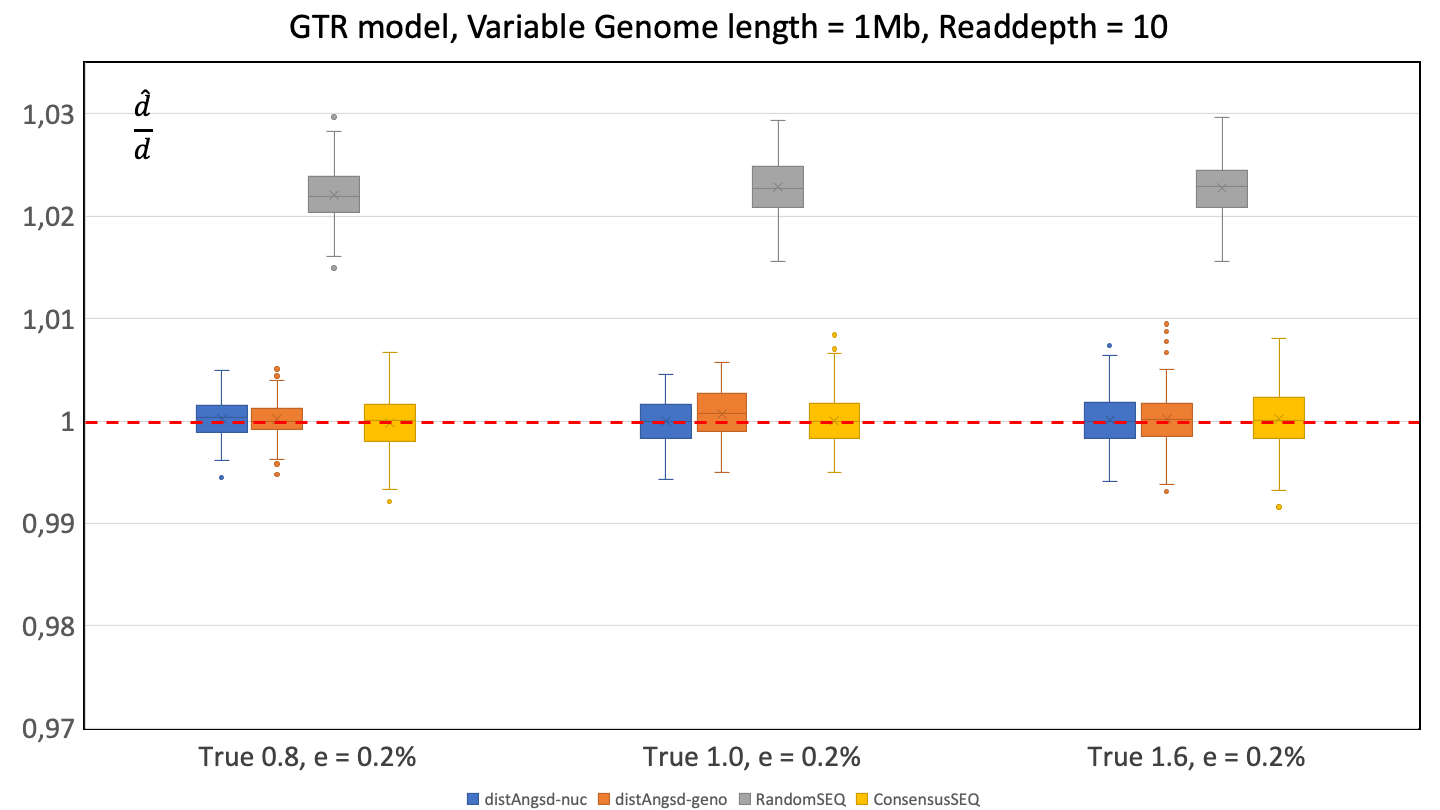
\includegraphics[width=\textwidth]{GTRRD10_1Mb.png}
         \caption{}
         \label{fig:GTRRD10_1Mb}
     \end{subfigure}
     \begin{subfigure}[b]{0.475\textwidth}
         \centering
         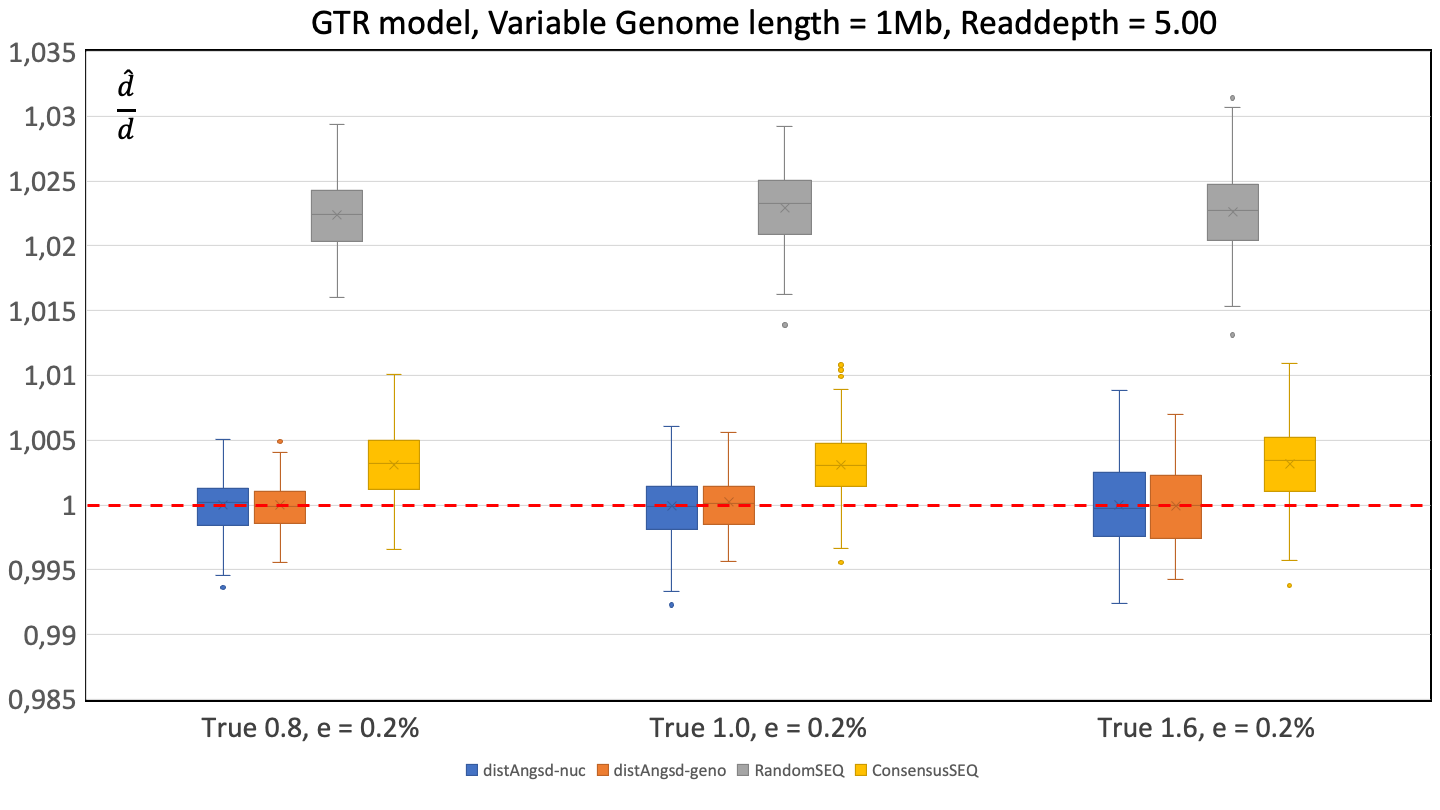
\includegraphics[width=\textwidth]{GTRRD5_1Mb.png}
         \caption{}
         \label{fig:GTRRD5_1Mb}
     \end{subfigure}
     \begin{subfigure}[b]{0.475\textwidth}
         \centering
         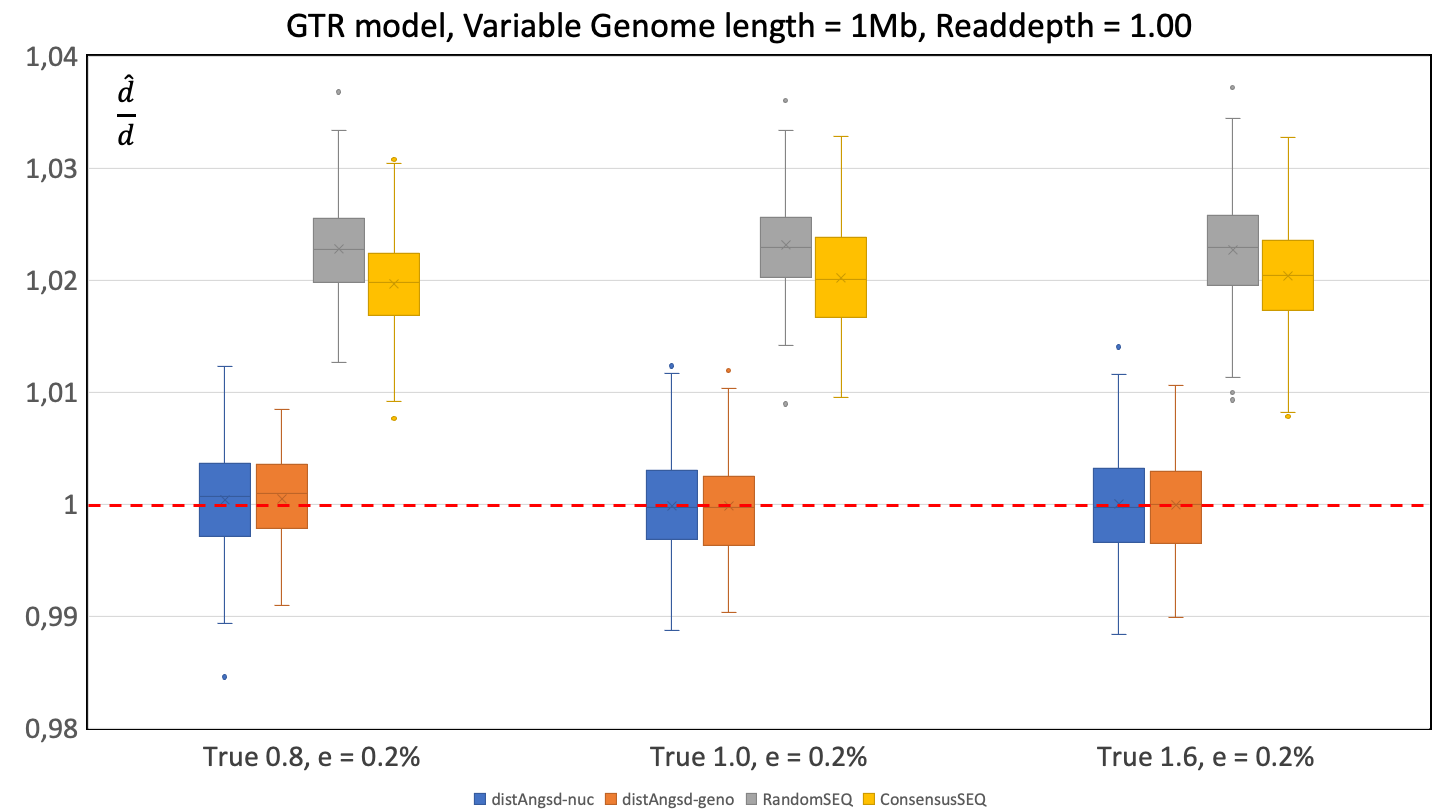
\includegraphics[width=\textwidth]{GTRRD1_1Mb.png}
         \caption{}
         \label{fig:GTRRD1_1Mb}
     \end{subfigure}
     \begin{subfigure}[b]{0.475\textwidth}
         \centering
         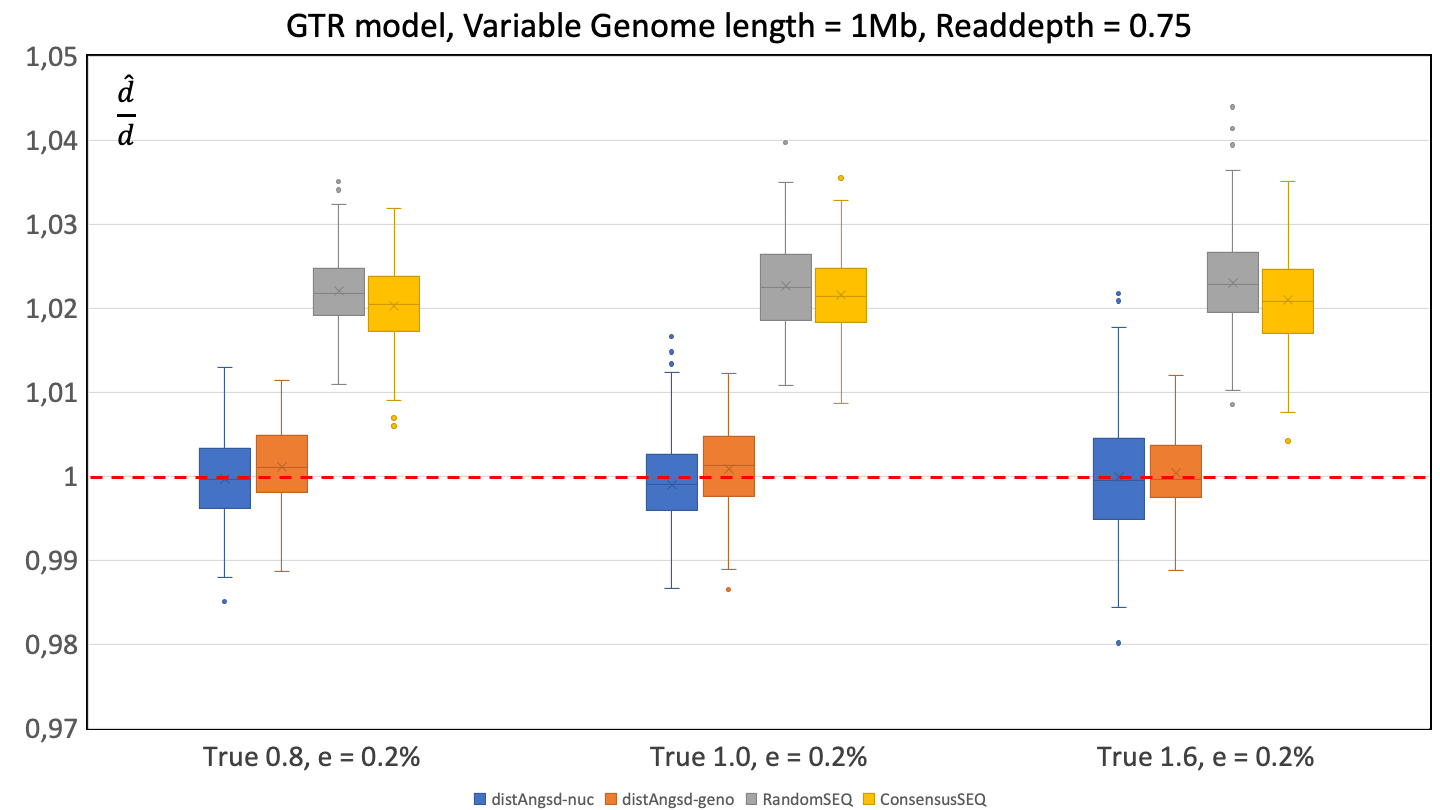
\includegraphics[width=\textwidth]{GTRRD075_1Mb.png}
         \caption{}
         \label{fig:GTRRD075_1Mb}
     \end{subfigure}
     \begin{subfigure}[b]{0.475\textwidth}
         \centering
         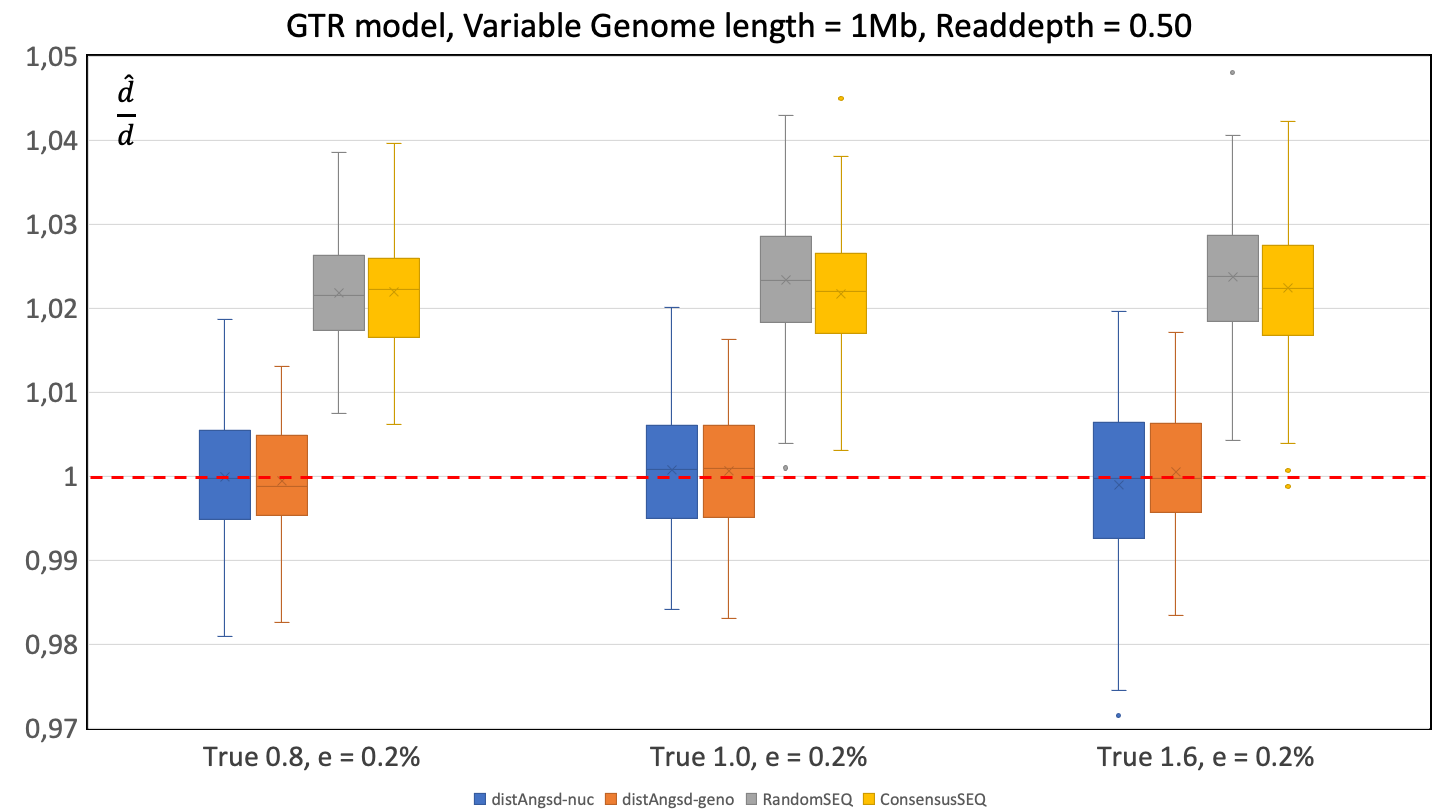
\includegraphics[width=\textwidth]{GTRRD05_1Mb.png}
         \caption{}
         \label{fig:GTRRD05_1Mb}
     \end{subfigure}
    \vspace{0.5cm}
    \caption{The inferred results of four different methods based $200$ replicates of GTR model simulation, i.e., distAngsd-nuc, distAngsd-geno, RandomSEQ, and ConsensusSEQ when genome length is $1$Mb, and the average read depth per site varies from (a) $20$ to (f) $0.5$. The simulated base calling error is $e =0.2\%$. Simulated divergence tree follows Fig. \ref{fig:basictree4inference}, with $t_1=0.4$ and $t_2 = 0.25$, and true simulated divergence time $t$ (hence the genetic distance $d$) is set as $0.8$, $1.0$ and $1.6$.}
    \label{fig:GTR1Mb}
\end{figure*}

% \begin{figure*}
%     \centering
%     \begin{subfigure}[b]{0.475\textwidth}
%          \centering
%          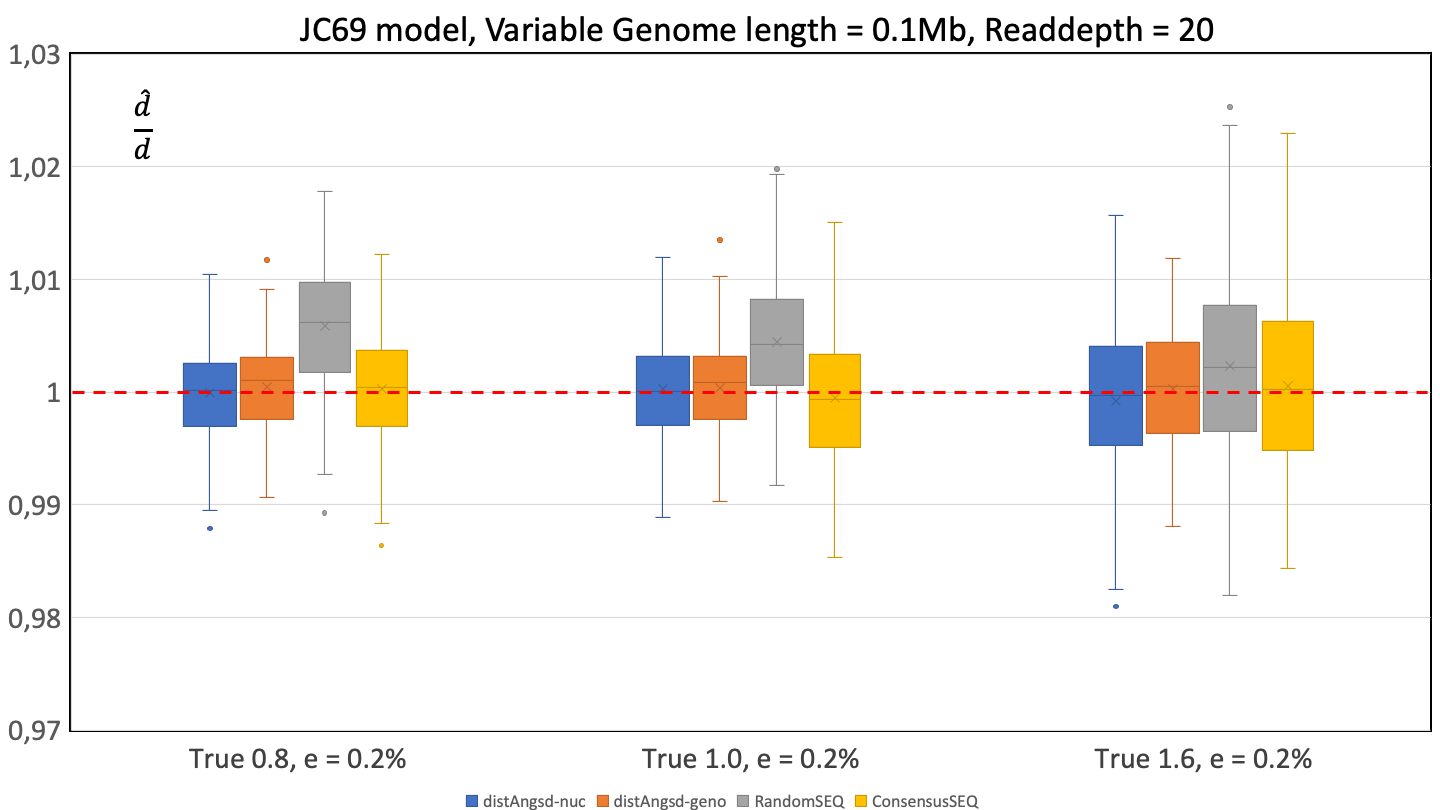
\includegraphics[width=\textwidth]{JCRD20_01Mb.png}
%          \caption{}
%          \label{fig:JCRD20_01Mb}
%      \end{subfigure}
%      \begin{subfigure}[b]{0.475\textwidth}
%          \centering
%          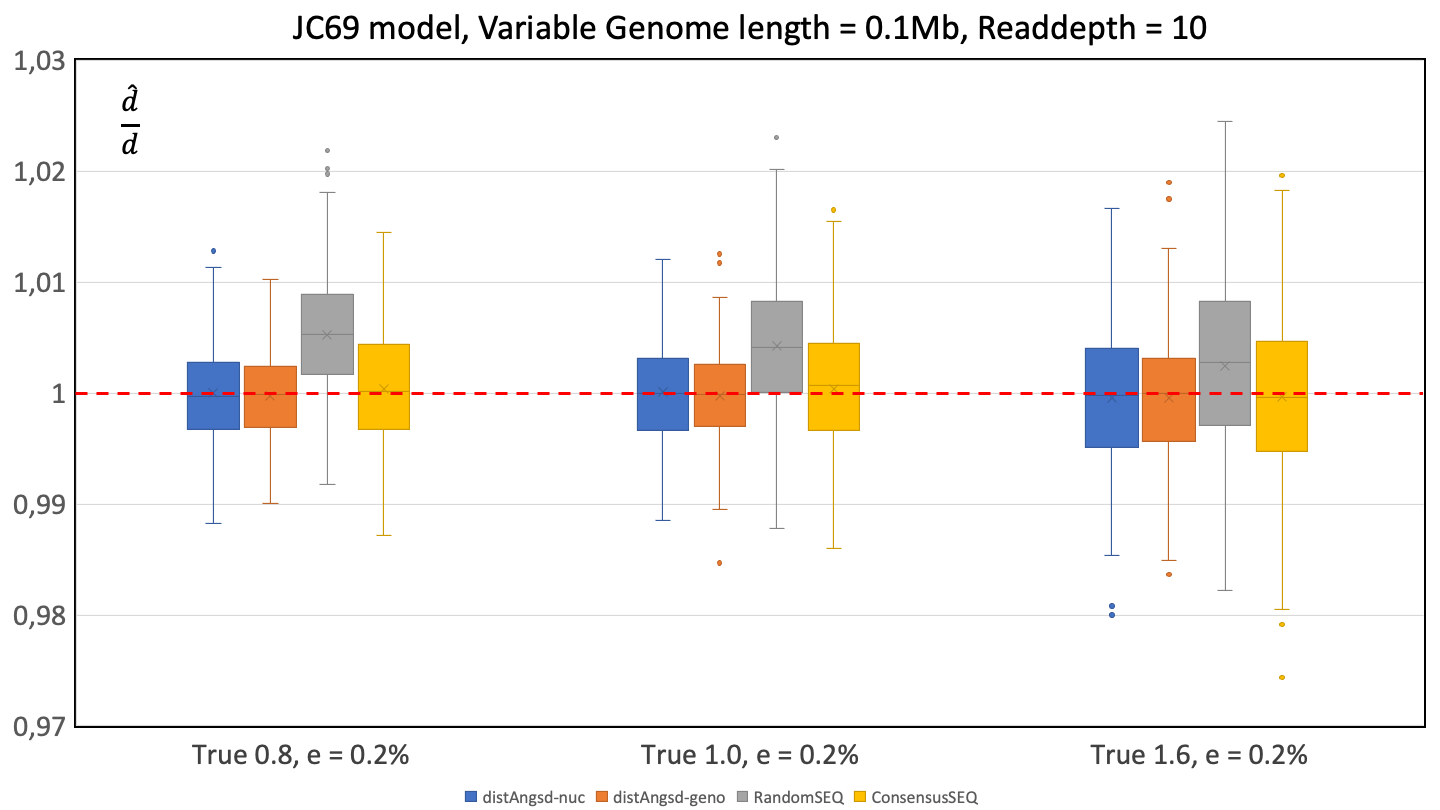
\includegraphics[width=\textwidth]{JCRD10_01Mb.png}
%          \caption{}
%          \label{fig:JCRD10_01Mb}
%      \end{subfigure}
%      \begin{subfigure}[b]{0.475\textwidth}
%          \centering
%          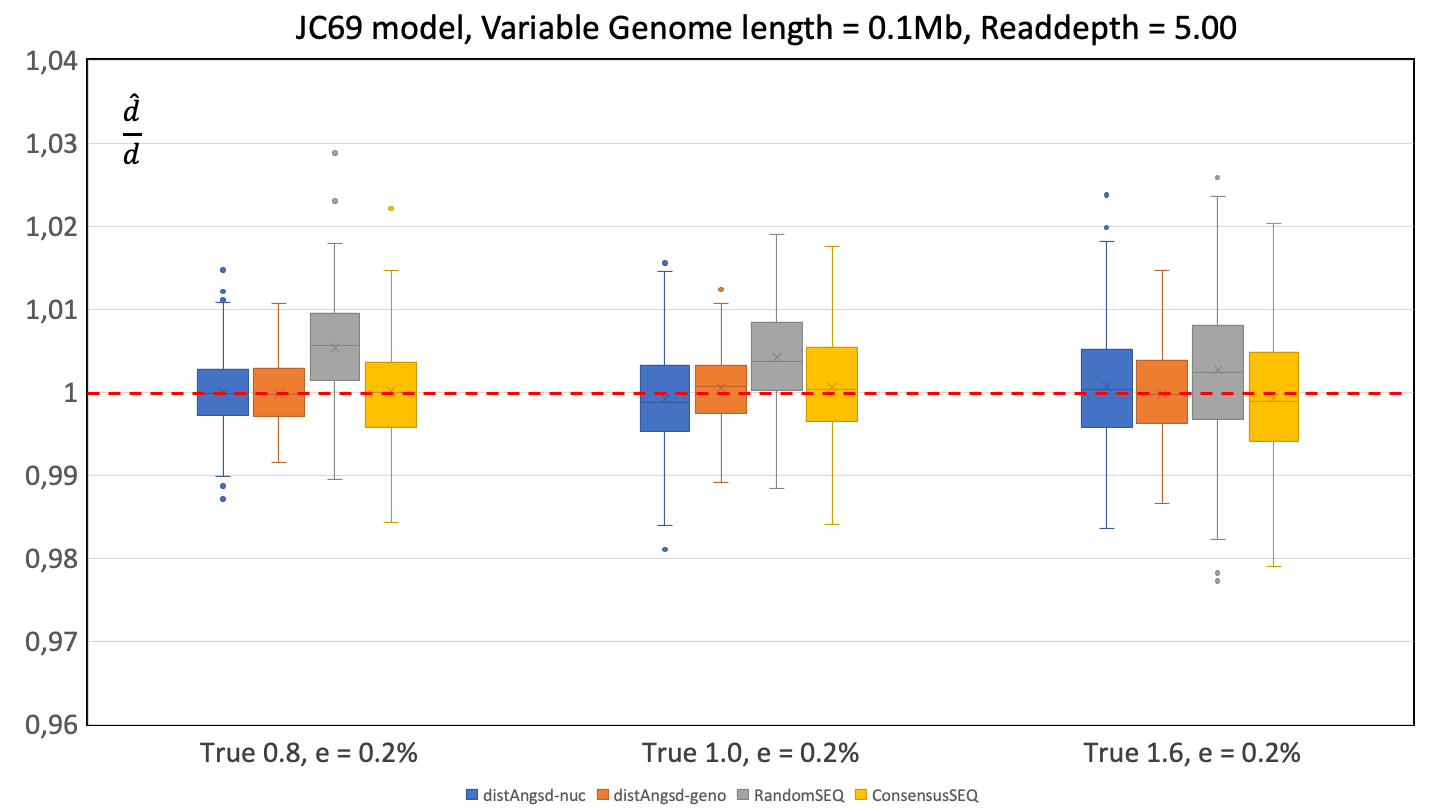
\includegraphics[width=\textwidth]{JCRD5_01Mb.png}
%          \caption{}
%          \label{fig:JCRD5_01Mb}
%      \end{subfigure}
%      \begin{subfigure}[b]{0.475\textwidth}
%          \centering
%          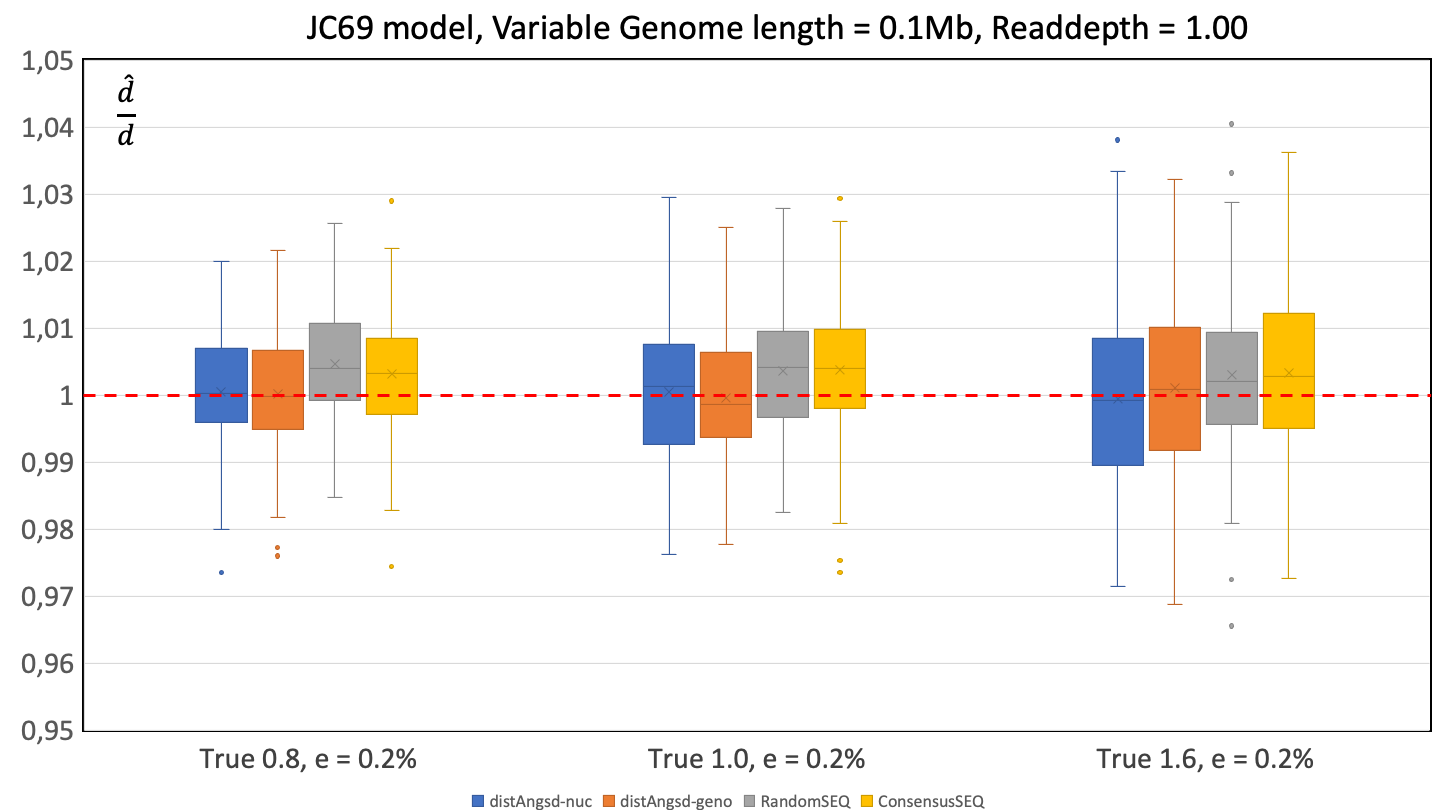
\includegraphics[width=\textwidth]{JCRD1_01Mb.png}
%          \caption{}
%          \label{fig:JCRD1_01Mb}
%      \end{subfigure}
%      \begin{subfigure}[b]{0.475\textwidth}
%          \centering
%          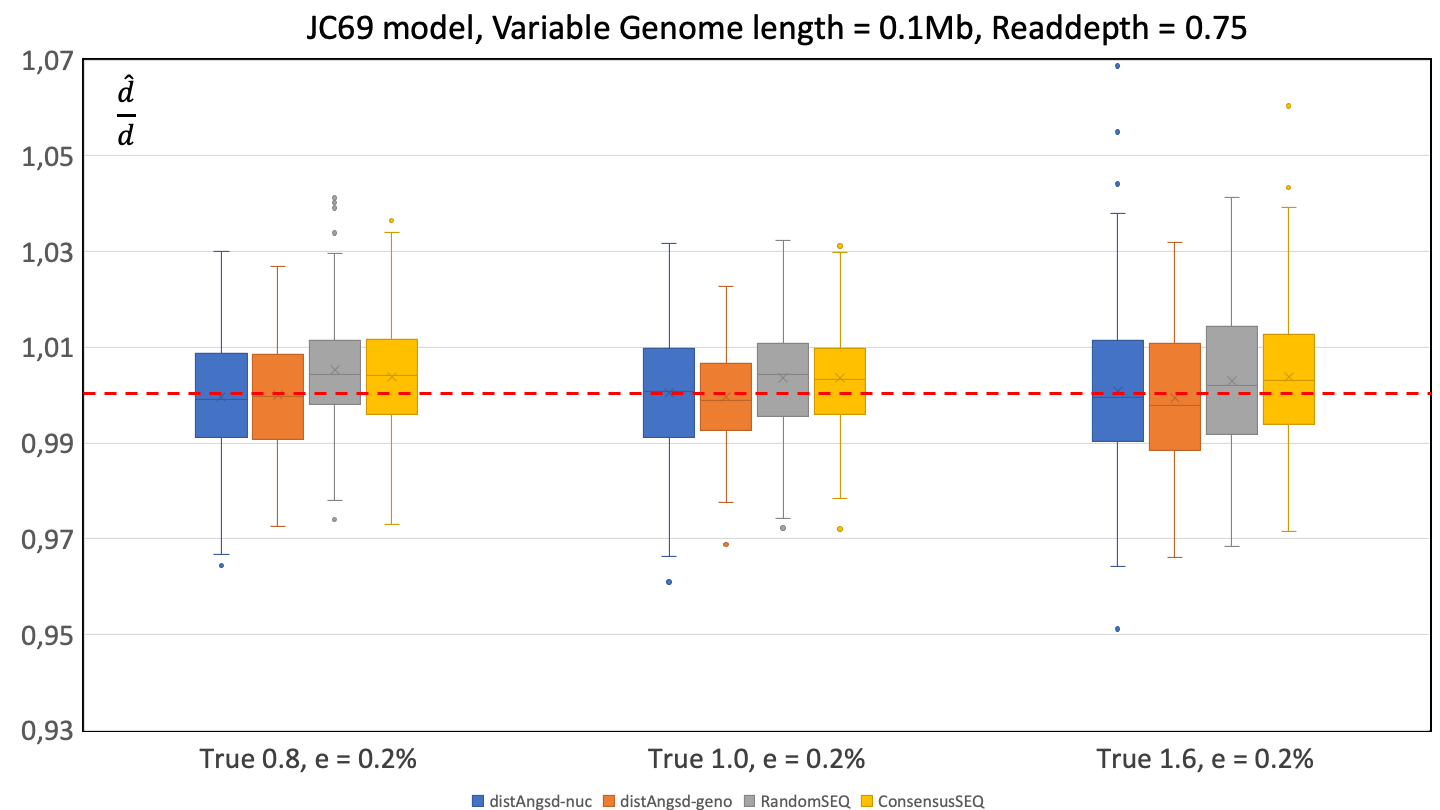
\includegraphics[width=\textwidth]{JCRD075_01Mb.png}
%          \caption{}
%          \label{fig:JCRD075_01Mb}
%     \end{subfigure}
%      \begin{subfigure}[b]{0.475\textwidth}
%          \centering
%          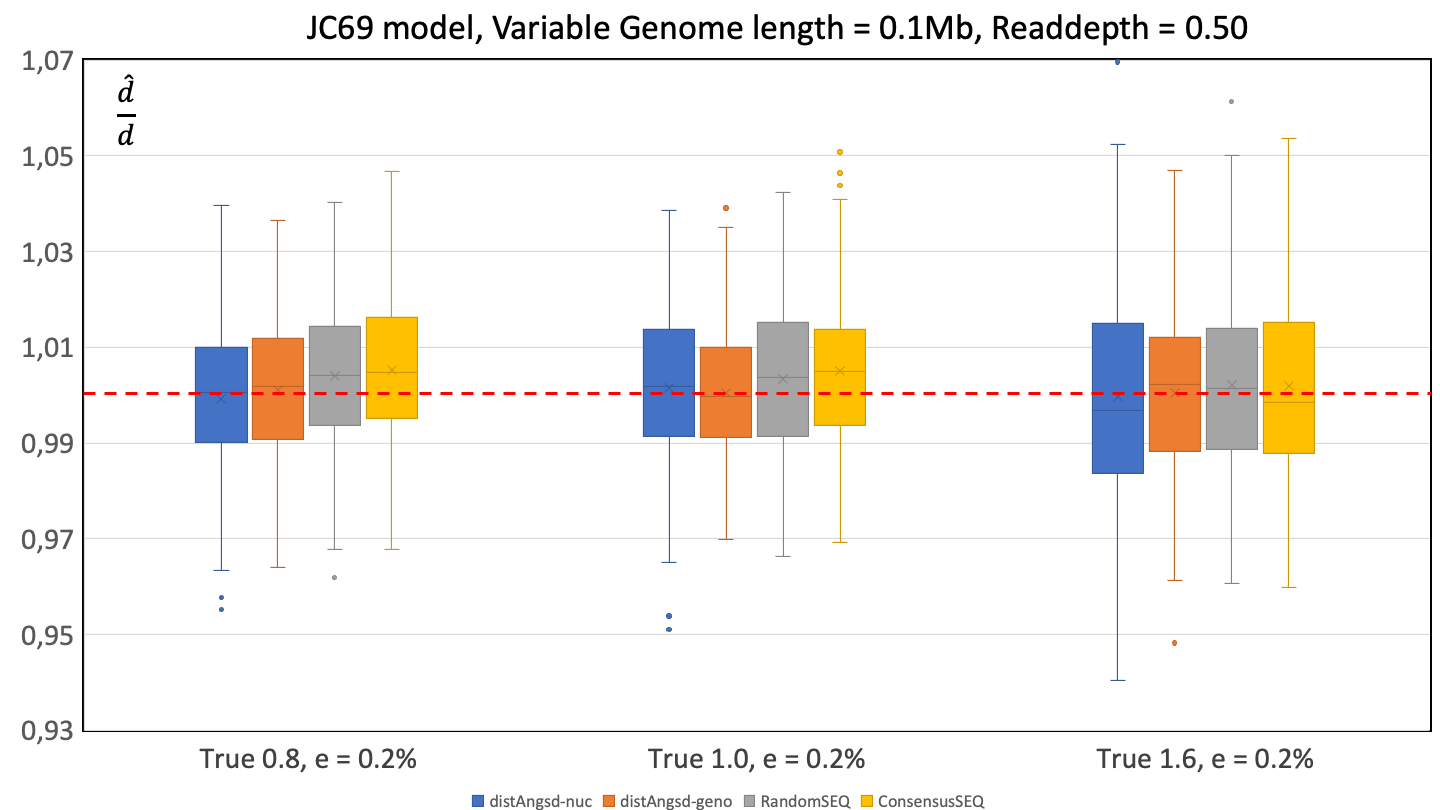
\includegraphics[width=\textwidth]{JCRD05_01Mb.png}
%          \caption{}
%          \label{fig:JCRD05_01Mb}
%     \end{subfigure}
%     \vspace{0.5cm}
%     \caption{The inferred results of four different methods based $200$ replicates of JC69 model simulation, i.e., distAngsd-nuc, distAngsd-geno, RandomSEQ, and ConsensusSEQ when genome length is $0.1$Mb, and the average read depth per site varies from (a) $20$ to (f) $0.5$. The simulated base calling error is $e =0.2\%$. Simulated divergence tree follows Fig. \ref{fig:basictree4inference}, with $t_1=0.4$ and $t_2 = 0.25$, and true simulated divergence time $t$ (hence the genetic distance $d$) is set as $0.8$, $1.0$ and $1.6$.}
%     \label{fig:JC01Mb}
% \end{figure*}

% \begin{figure*}
%     \centering
%         \begin{subfigure}[b]{0.475\textwidth}
%          \centering
%          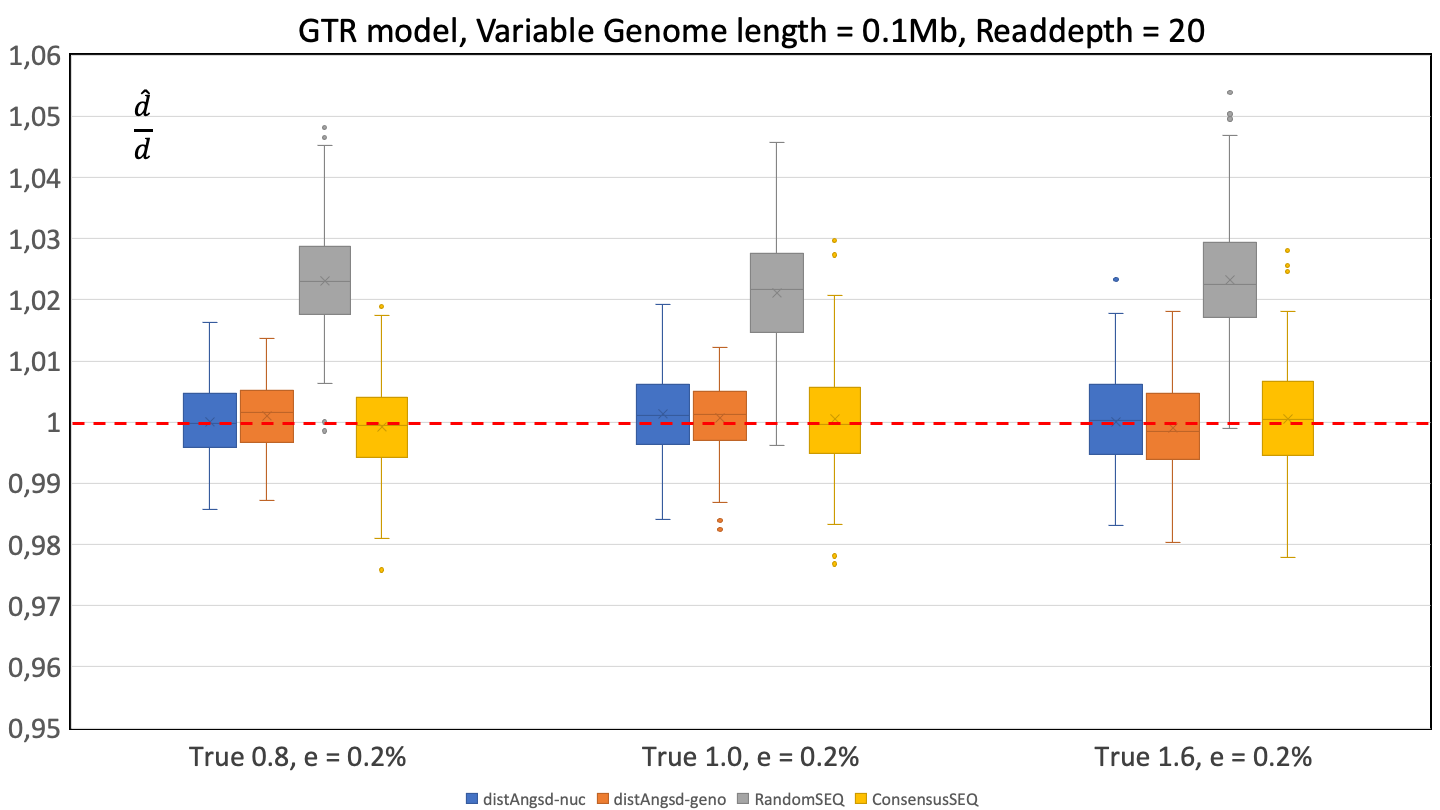
\includegraphics[width=\textwidth]{GTRRD20_01Mb.png}
%          \caption{}
%          \label{fig:GTRRD20_01Mb}
%      \end{subfigure}
%      \begin{subfigure}[b]{0.475\textwidth}
%          \centering
%          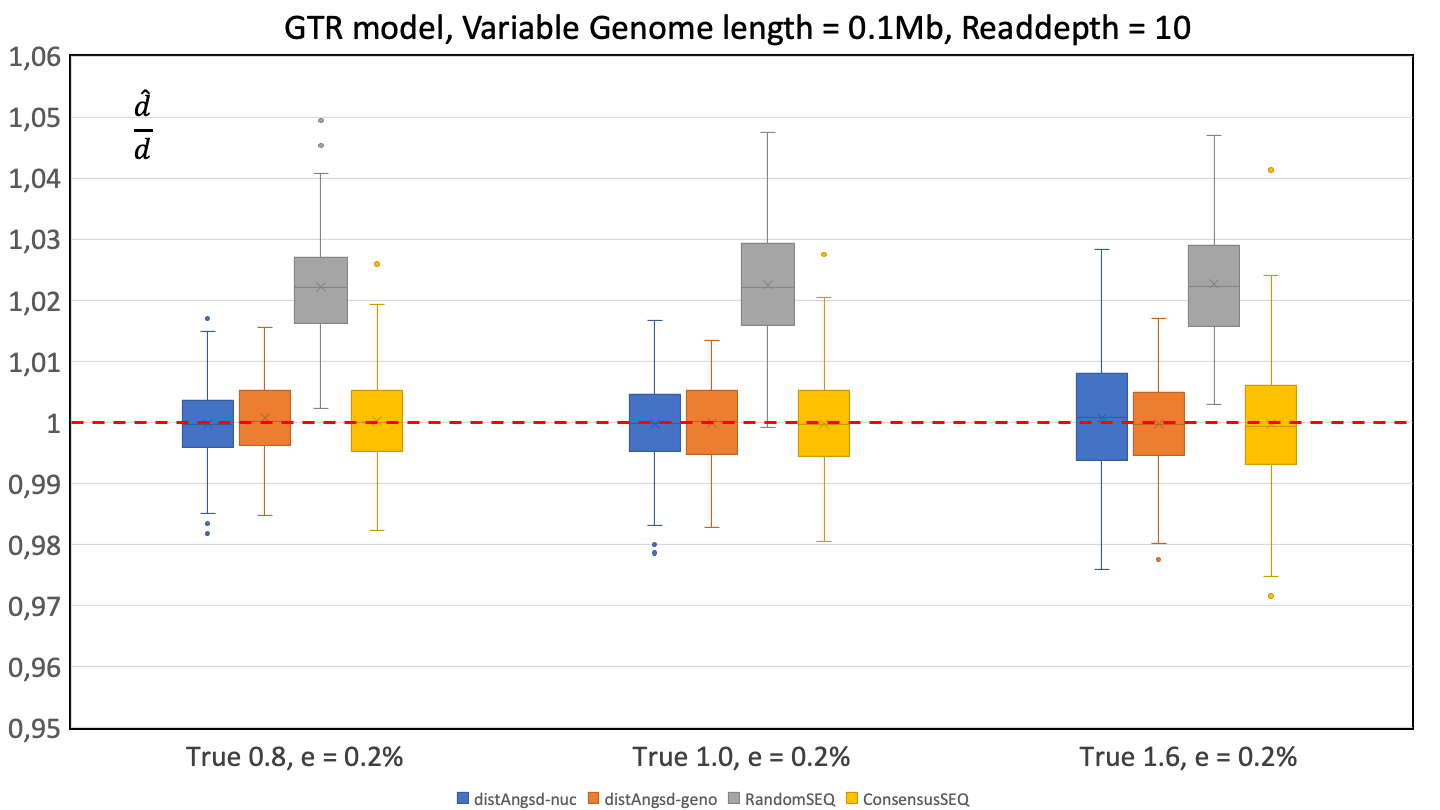
\includegraphics[width=\textwidth]{GTRRD10_01Mb.png}
%          \caption{}
%          \label{fig:GTRRD10_01Mb}
%      \end{subfigure}
%      \begin{subfigure}[b]{0.475\textwidth}
%          \centering
%          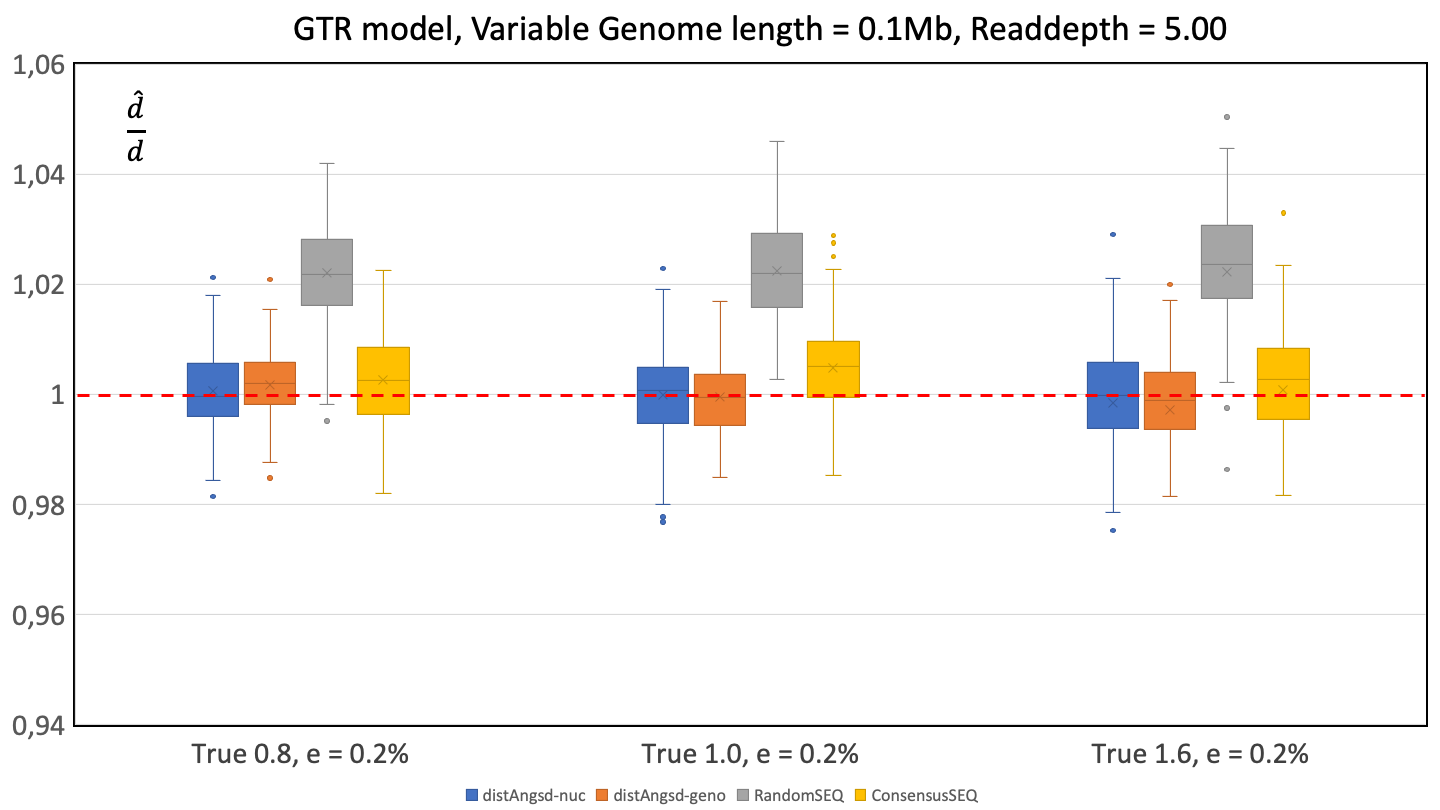
\includegraphics[width=\textwidth]{GTRRD5_01Mb.png}
%          \caption{}
%          \label{fig:GTRRD5_01Mb}
%      \end{subfigure}
%      \begin{subfigure}[b]{0.475\textwidth}
%          \centering
%          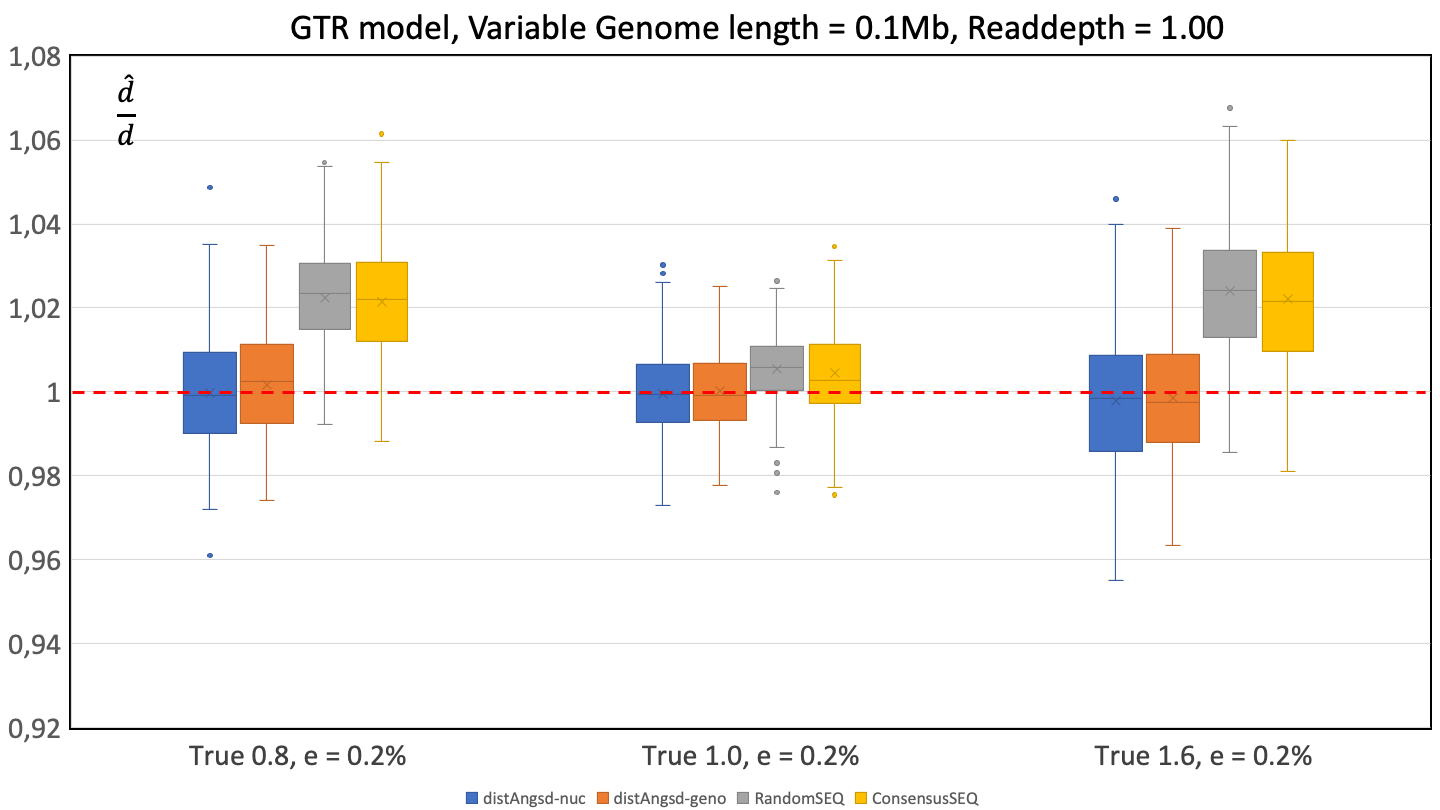
\includegraphics[width=\textwidth]{GTRRD1_01Mb.png}
%          \caption{}
%          \label{fig:GTRRD1_01Mb}
%      \end{subfigure}
%      \begin{subfigure}[b]{0.475\textwidth}
%          \centering
%          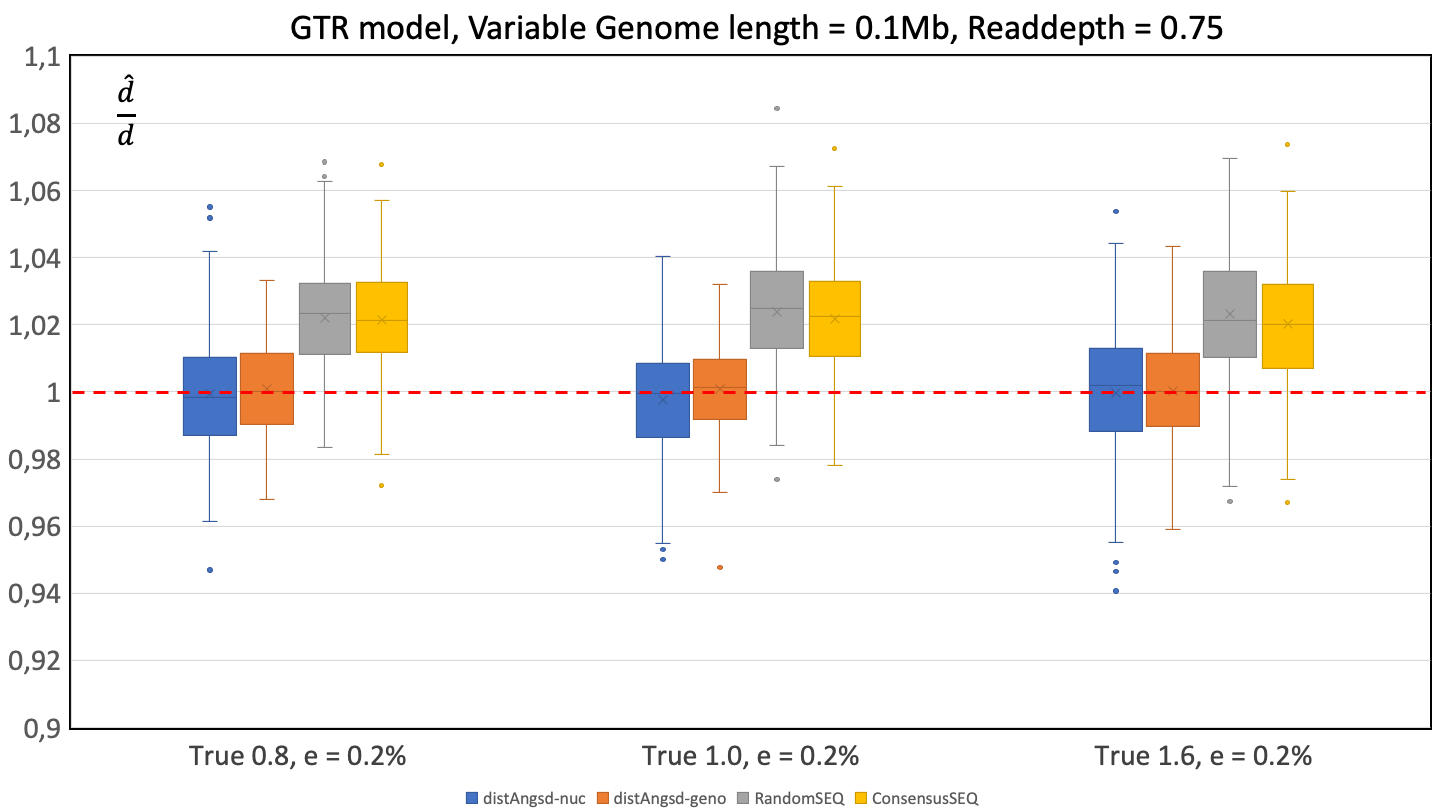
\includegraphics[width=\textwidth]{GTRRD075_01Mb.png}
%          \caption{}
%          \label{fig:GTRRD075_01Mb}
%      \end{subfigure}
%      \begin{subfigure}[b]{0.475\textwidth}
%          \centering
%          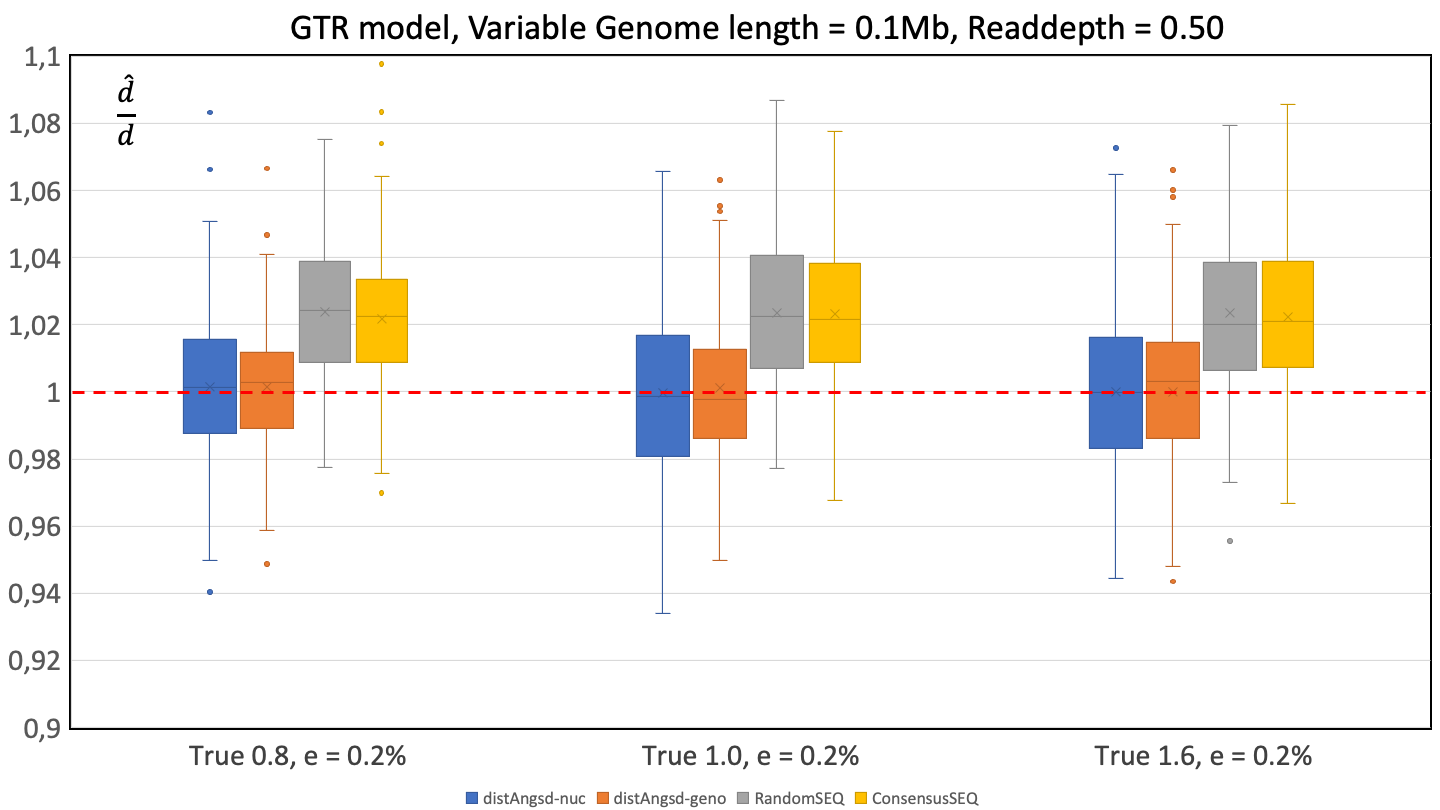
\includegraphics[width=\textwidth]{GTRRD05_01Mb.png}
%          \caption{}
%          \label{fig:GTRRD05_01Mb}
%      \end{subfigure}
%     \vspace{0.5cm}
%     \caption{The inferred results of four different methods based $200$ replicates of GTR model simulation, i.e., distAngsd-nuc, distAngsd-geno, RandomSEQ, and ConsensusSEQ when genome length is $0.1$Mb, and the average read depth per site varies from (a) $20$ to (f) $0.5$. The simulated base calling error is $e =0.2\%$. Simulated divergence tree follows Fig. \ref{fig:basictree4inference}, with $t_1=0.4$ and $t_2 = 0.25$, and true simulated divergence time $t$ (hence the genetic distance $d$) is set as $0.8$, $1.0$ and $1.6$.}
%     \label{fig:GTR01Mb}
% \end{figure*}

Compared with the pre-existing methods, both distAngsd-geno and distAngsd-nuc have the fewer biases in the inference especially when less data is present (lower read depth, see FIG. \ref{fig:JC1Mb} and FIG. \ref{fig:GTR1Mb} or shorter variable genome length, compared with FIG. S8 and FIG. S9 in Supplementary Information). but for the inferences based on extremely poor data, we remind readers that both of our methods can also be biased, which is discussed in the Supplementary Information. And when the genetic data per sample is large enough, as the our methods take advantage of all reads information and base calling error profile, they normally have the smallest variance in inference. And since distAngsd-geno also uses the prior knowledge of ploidy level, it always has the inference results with least variances.

As in this part, only variable sites are taken into consideration, a large proportion of sites are heterozygous,  essential impacts will be imposed on the ConsensusGT by the ambiguous inference method, which makes its results relatively far away from the true simulated parameter $d$. ConsensusGT results of variable genome length $1$Mbp are plotted in FIG. \ref{fig:JC1Mb} and FIG. \ref{fig:GTR1Mb}, but instead are given in Table \ref{tab:ConsensusGT} (A similar table of variable genome $0.1$Mbp is given in Supplementary Information). As mean read depth becomes lower and lower, the ConsensusGT inferred genetic distance of becomes larger and larger, and closer to the true $d$. This is due to that more heterozygous sites will be misclassified as homogeneous sites, and the ambiguous inference, which will always underestimate $d$ in presence of heterozygous sites, becomes less biased.


\begin{table*}[ht]
    \centering
    \begin{tabular}{|c|c|c|c|c|c|c|}
     \hline
      \multirow{3}{*}{Average Read Depth} & \multicolumn{6}{c|}{Mean of Inferred $\hat{d}$}\\
      &\multicolumn{2}{c|}{True $d$: $0.8000$}&\multicolumn{2}{c|}{True $d$: $1.000$}&\multicolumn{2}{c|}{True $d$: $1.600$}\\
      &JC69&GTR&JC69&GTR&JC69&GTR\\
      \hline
      $20$  & $0.3149$ &$0.3119$& $0.5122$ & $0.4870$ & $1.105$ & $1.011$\\
      \hline
      $10$  & $0.3229$ & $0.3206$ & $0.5204$ & $0.4957$ & $1.114$ & $1.020$\\
      \hline
      $5$  & $0.3941$ & $0.3949$ & $0.5926$ & $0.5725$ & $1.188$ & $1.107$\\
      \hline
      $1$  & $0.6900$ & $0.6983$ & $0.8907$ & $0.8931$ & $1.492$ & $1.480$\\
       \hline
      $0.75$ & $0.7180$ & $0.7265$ & $0.9186$ & $0.9246$ & $0.9186$ & $1.517$\\
      \hline
      $0.5$  & $0.7459$ & $0.7571$ & $0.9465$ & $0.9565$ & $1.548$ & $1.557$\\
      \hline
      \end{tabular}
    \caption{ConsensusGT inferred results based on 200 replicates of simulations of different models with variable genome length $1$Mb.}
    \label{tab:ConsensusGT}
\end{table*}

% \begin{table*}[ht]
%     \centering
%     \begin{tabular}{|c|c|c|c|c|c|c|c|}
%      \hline
%       \multirow{3}{*}{Average Read Depth} & \multirow{3}{*}{Variable Genome Length(Mb)} & \multicolumn{6}{c|}{Inferred $\hat{d}$}\\
%       &&\multicolumn{2}{c|}{True $d$: $0.8000$}&\multicolumn{2}{c|}{True $d$: $1.000$}&\multicolumn{2}{c|}{True $d$: $1.600$}\\
%       &&JC69&GTR&JC69&GTR&JC69&GTR\\
%       \hline
%       \multirow{2}{*}{$20$} & $0.1$ & $0.3147$ & $0.3124$ & $0.5118$ & $0.4866$ & $1.105$ & $1.012$\\
%       & $1$ & $0.3149$ &$0.3119$& $0.5122$ & $0.4870$ & $1.105$ & $1.011$\\
%       \hline
%       \multirow{2}{*}{$10$} & $0.1$ & $0.3228$ & $0.3207$ & $0.5204$ & $0.4957$ & $1.114$ & $1.020$\\
%       & $1$ & $0.3229$ & $0.3206$ & $0.5204$ & $0.4957$ & $1.114$ & $1.020$\\
%       \hline
%       \multirow{2}{*}{$5$} & $0.1$ & $0.3941$ & $0.3953$ & $0.5922$ & $0.5722$ & $1.188$ & $1.107$\\
%       & $1$ & $0.3941$ & $0.3949$ & $0.5926$ & $0.5725$ & $1.188$ & $1.107$\\
%       \hline
%       \multirow{2}{*}{$1$} & $0.1$ & $0.6903$ & $0.6998$ & $0.8912$ & $0.8911$ & $1.493$ & $1.482$\\
%       & $1$ & $0.6900$ & $0.6983$ & $0.8907$ & $0.8931$ & $1.492$ & $1.480$\\
%       \hline
%       \multirow{2}{*}{$0.75$} & $0.1$ & $0.7174$ & $0.7274$ & $0.9195$ & $0.9245$ & $1.520$ & $1.520$\\
%       & $1$ & $0.7180$ & $0.7265$ & $0.9186$ & $0.9246$ & $0.9186$ & $1.517$\\
%       \hline
%       \multirow{2}{*}{$0.5$} & $0.1$ & $0,7475$ & $0.7579$ & $0,9478$ & $0.9599$ & $1,547$ & $1.561$\\
%       & $1$ & $0.7459$ & $0.7571$ & $0.9465$ & $0.9565$ & $1.548$ & $1.557$\\
%       \hline
%       \end{tabular}
%     \caption{ConsensusGT inferred results based on 200 replicates of simulations of different models.}
%     \label{tab:ConsensusGT}
% \end{table*}

% \begin{table*}
%     \centering
%     \begin{tabular}{|l|ccc|}
%      \hline
%       \diagbox{\small Cases}{\small Inferred $\bar{\hat{d}}$}{\small True $d$} & $0.8000$ & $1.000$ & $1.600$\\
%       \hline
%       \small JC69, $\mathrm{RD}=20$, $\mathrm{GL}=1.0$Mb & \small 0.3149 & \small 0.5122 & \small 1.105\\
%       \small GTR, $\mathrm{RD}=20$, $\mathrm{GL}=1.0$Mb & \small 0.3119	& \small 0.4870 & \small 	1.011\\
%       \small JC69, $\mathrm{RD}=20$, $\mathrm{GL}=0.1$Mb & \small 0.3147 & \small 0.5118 & \small 1.105\\
%       \small GTR, $\mathrm{RD}=20$, $\mathrm{GL}=0.1$Mb & \small 0.3124	& \small 0.4866 & \small 1.012\\
%       \small JC69, $\mathrm{RD}=10$, $\mathrm{GL}=1.0$Mb & \small 0.3229 & \small 0.5204 & \small 1.114\\
%       \small GTR, $\mathrm{RD}=10$, $\mathrm{GL}=1.0$Mb & \small 0.3206	& \small 0.4957 & \small 1.020\\
%       \small JC69, $\mathrm{RD}=10$, $\mathrm{GL}=0.1$Mb & \small 0.3228	& \small 0.5204	& \small 1.114\\
%       \small GTR, $\mathrm{RD}=10$, $\mathrm{GL}=0.1$Mb & \small 0.3207 & \small 0.4957 & \small 1.020\\
%       \small JC69, $\mathrm{RD}=5$, $\mathrm{GL}=1.0$Mb & \small 0.3941	& \small 0.5926& \small 1.188\\
%       \small GTR, $\mathrm{RD}=5$, $\mathrm{GL}=1.0$Mb & \small 0.3949	& \small 0.5725 & \small 1.107\\
%       \small JC69, $\mathrm{RD}=5$, $\mathrm{GL}=0.1$Mb & \small 0.3941	& \small 0.5922& \small 1.188\\
%       \small GTR, $\mathrm{RD}=5$, $\mathrm{GL}=0.1$Mb & \small 0.3953 & \small 0.5722 & \small 1.107\\
%       \small JC69, $\mathrm{RD}=1$, $\mathrm{GL}=1.0$Mb & \small 0.6900	& \small 0.8907 & \small 1.492\\
%       \small GTR, $\mathrm{RD}=1$, $\mathrm{GL}=1.0$Mb & \small 0.6983 & \small 0.8931 & \small 1.480\\
%       \small JC69, $\mathrm{RD}=1$, $\mathrm{GL}=0.1$Mb & \small 0.6903	& \small 0.8912& \small 1.493\\
%       \small GTR, $\mathrm{RD}=1$, $\mathrm{GL}=0.1$Mb & \small 0.6998 & \small 0.8911 & \small 1.482\\
%       \small JC69, $\mathrm{RD}=0.75$, $\mathrm{GL}=1.0$Mb & \small 0.7180 & \small 0.9186& \small 	1.520\\
%       \small GTR, $\mathrm{RD}=0.75$, $\mathrm{GL}=1.0$Mb & \small 0.7265  & \small 0.9246& \small 1.517\\
%       \small JC69, $\mathrm{RD}=0.75$, $\mathrm{GL}=0.1$Mb & \small 0.7174 & \small 0.9195 & \small 1.520\\
%       \small GTR, $\mathrm{RD}=0.75$, $\mathrm{GL}=0.1$Mb & \small 0.7274 & \small 0.9245 & \small 1.520\\
%       \small JC69, $\mathrm{RD}=0.5$, $\mathrm{GL}=1.0$Mb & \small 0.7459 & \small 0.9465 & \small 1.548\\
%       \small GTR, $\mathrm{RD}=0.5$, $\mathrm{GL}=1.0$Mb & \small 0.7571 & \small 0.9565 & \small 1.557\\
%       \small JC69, $\mathrm{RD}=0.5$, $\mathrm{GL}=0.1$Mb & \small 0,7475 & \small 0,9478& \small 1,547\\
%       \small GTR, $\mathrm{RD}=0.5$, $\mathrm{GL}=0.1$Mb & \small 0.7579 & \small 0.9599 & \small 1.561\\
%       \hline
%       \end{tabular}
%     \caption{ConsensusGT inferred results based on 200 replicates of simulations of different models. In the table,
%     $\mathrm{RD}$ represents mean of read depth within the sample, while $\mathrm{GL}$ is the variable genome length.}
%     \label{tab:ConsensusGT}
% \end{table*}

{\color{red} As NGSDist could not distinguish different types of nucleotide substitutions, we only compare the inferred results of NGSDist and disAngsd-geno base on the JC69 model (FIG. \ref{fig:NGSdistdd}). NGSdist results $\hat{d}_{\mathrm{ngsDist}}$ is a nonlinear monotonically increasing function of the true $d$, and the curve is bending down as the true genetic distance becomes larger which reflects the infinite sites model that NGSDist adopts and no recurrent mutation is allowed. With the above comparisons, we draw the conclusion that the genetic distance measurement of NGSDist is evolutionary model-free, but may lose some power when inferring deep phylogenetic topology.

Since both NGSDist and disAngsd-geno are based on geotype likelihoods, the inferred genetic distances are expected to fluctuate around its true value as the mean read depth varies from $0.25$ to $20$. Such comparison is given in FIG. S10 of Supplementary Information, which shows the results of disAngsd-geno are more stable than those of NGSDist.
}
\begin{figure}[ht]
    \centering
         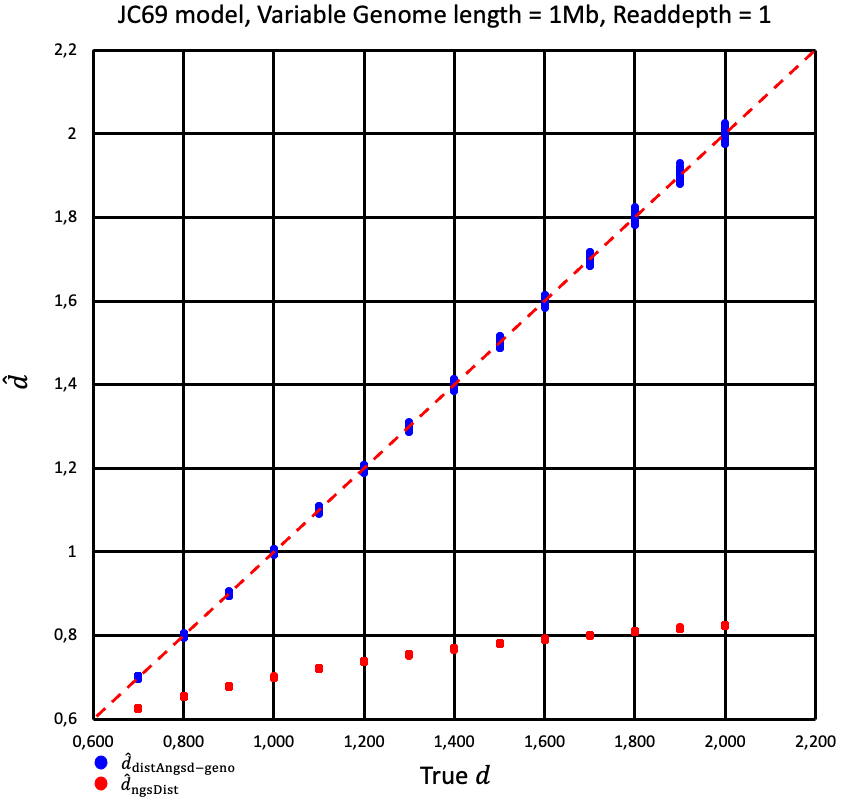
\includegraphics[width=0.95\columnwidth]{squaredd.png}
         \vspace{0.25cm}
         \caption{JC69 model is simulated to compare the inference results of distAngsd-geno and ngsDist. The average read depth is $1$ for all the simulations. Each point cluster represents 200 simulations with true genetic distance $d$ 0.7, 0.8, 0.9, 1.0, 1.1, 1.2, 1.3, 1.4, 1.5, 1.6, 1.7, 1.8, 1.9 or 2.0 (follows divergence tree as Fig. \ref{fig:basictree4inference}, with $t_1=0.4$ and $t_2 = 0.25$). And both ngsDist and distAngsd are conducted for each simulated result, {\tiny $(d,\hat{d}_{\mathrm{distAngsd}−-\mathrm{geno}})$} are plotted as the blue points, while {\tiny $(d,\hat{d}_{\mathrm{ngsDist}})$} are plotted as the red points.}
         \label{fig:NGSdistdd}
\end{figure}
% \begin{figure*}
%     \centering
%         \begin{subfigure}[b]{0.475\textwidth}
%          \centering
%          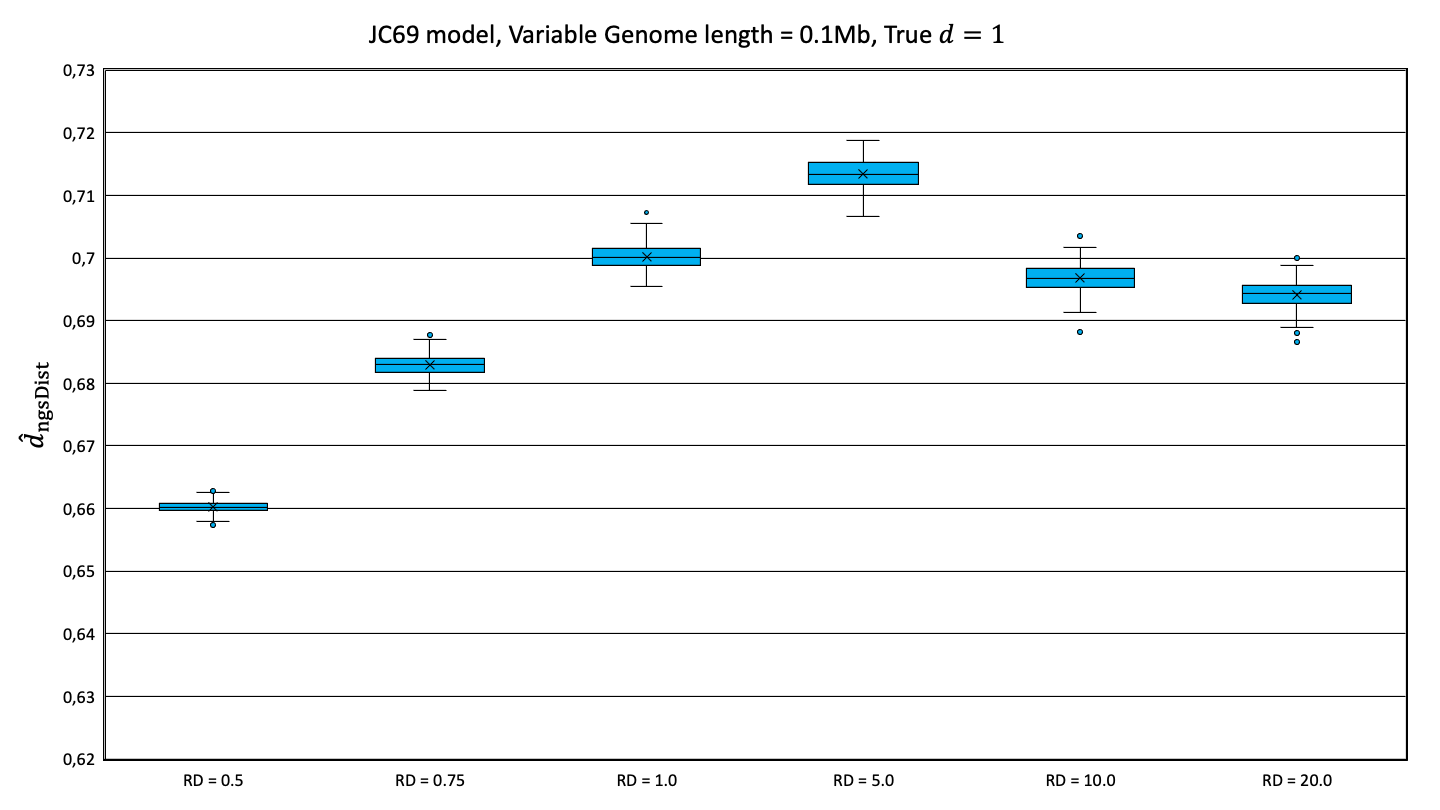
\includegraphics[width=\textwidth]{NGSdist01Mb.png}
%          \caption{}
%          \label{fig:NGSdistRD01Mb}
%      \end{subfigure}
%      \begin{subfigure}[b]{0.475\textwidth}
%          \centering
%          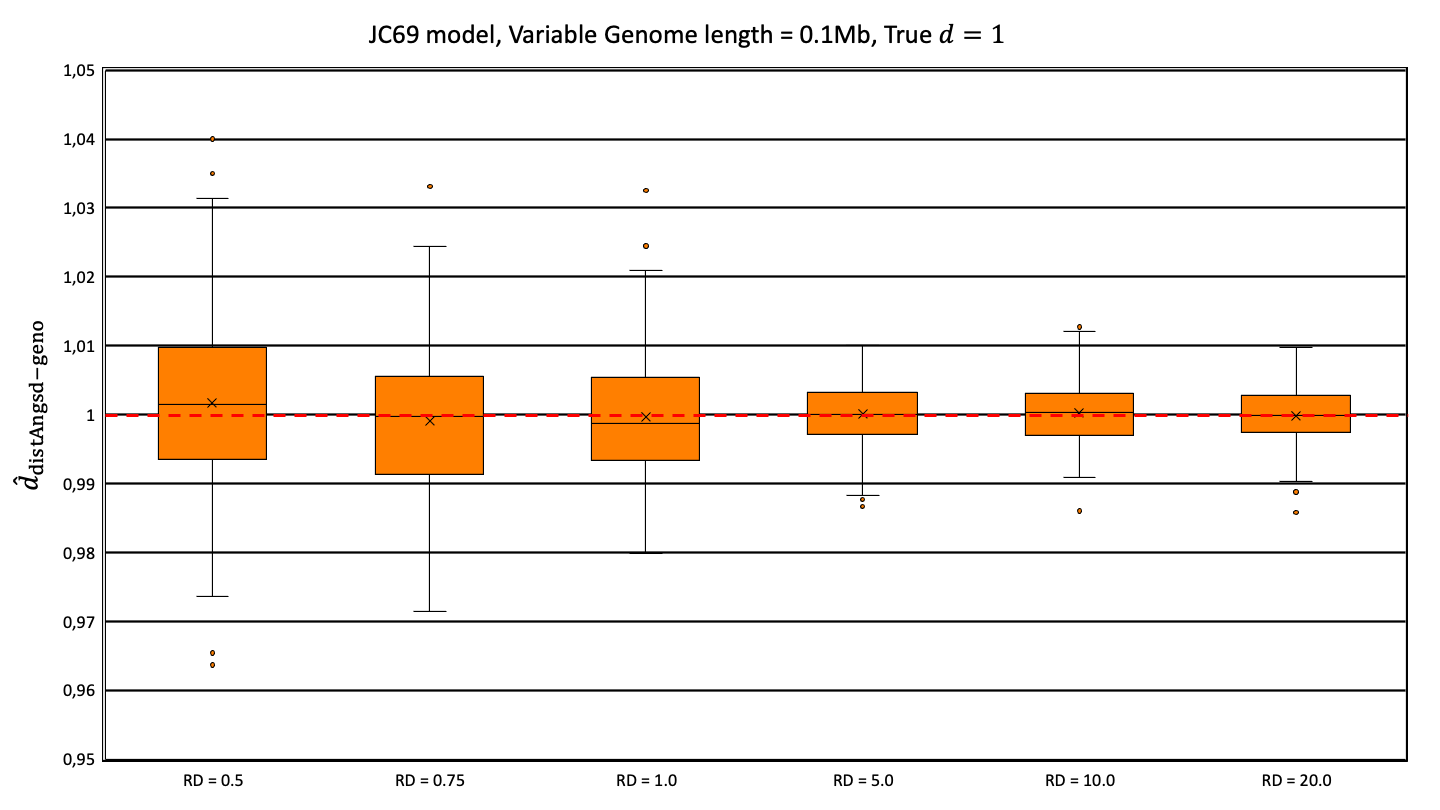
\includegraphics[width=\textwidth]{distAngsd-geno01Mb.png}
%          \caption{}
%          \label{fig:distAngsd-genoRD01Mb}
%      \end{subfigure}
%         \begin{subfigure}[b]{0.475\textwidth}
%          \centering
%          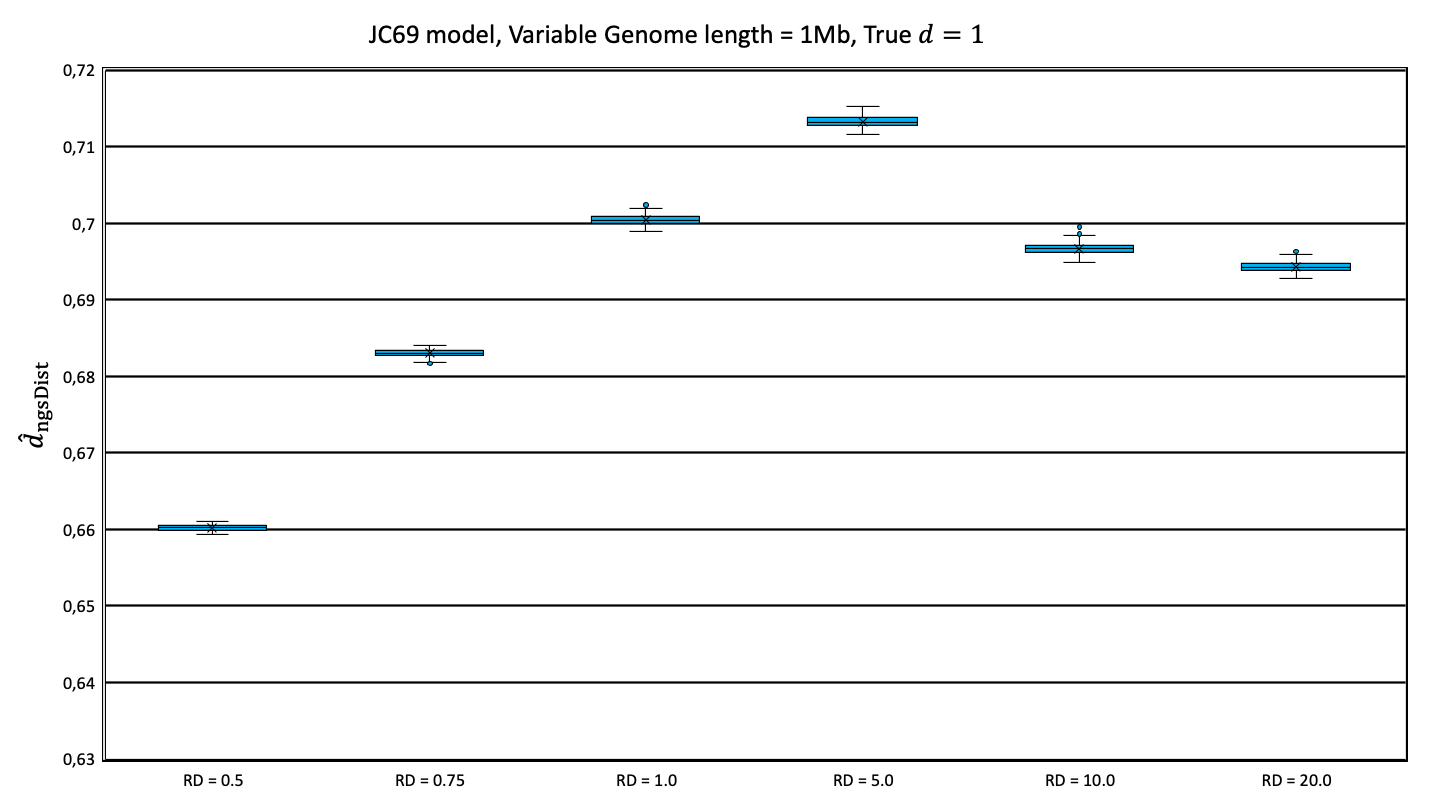
\includegraphics[width=\textwidth]{NGSdist.png}
%          \caption{}
%          \label{fig:NGSdist}
%      \end{subfigure}
%      \begin{subfigure}[b]{0.475\textwidth}
%          \centering
%          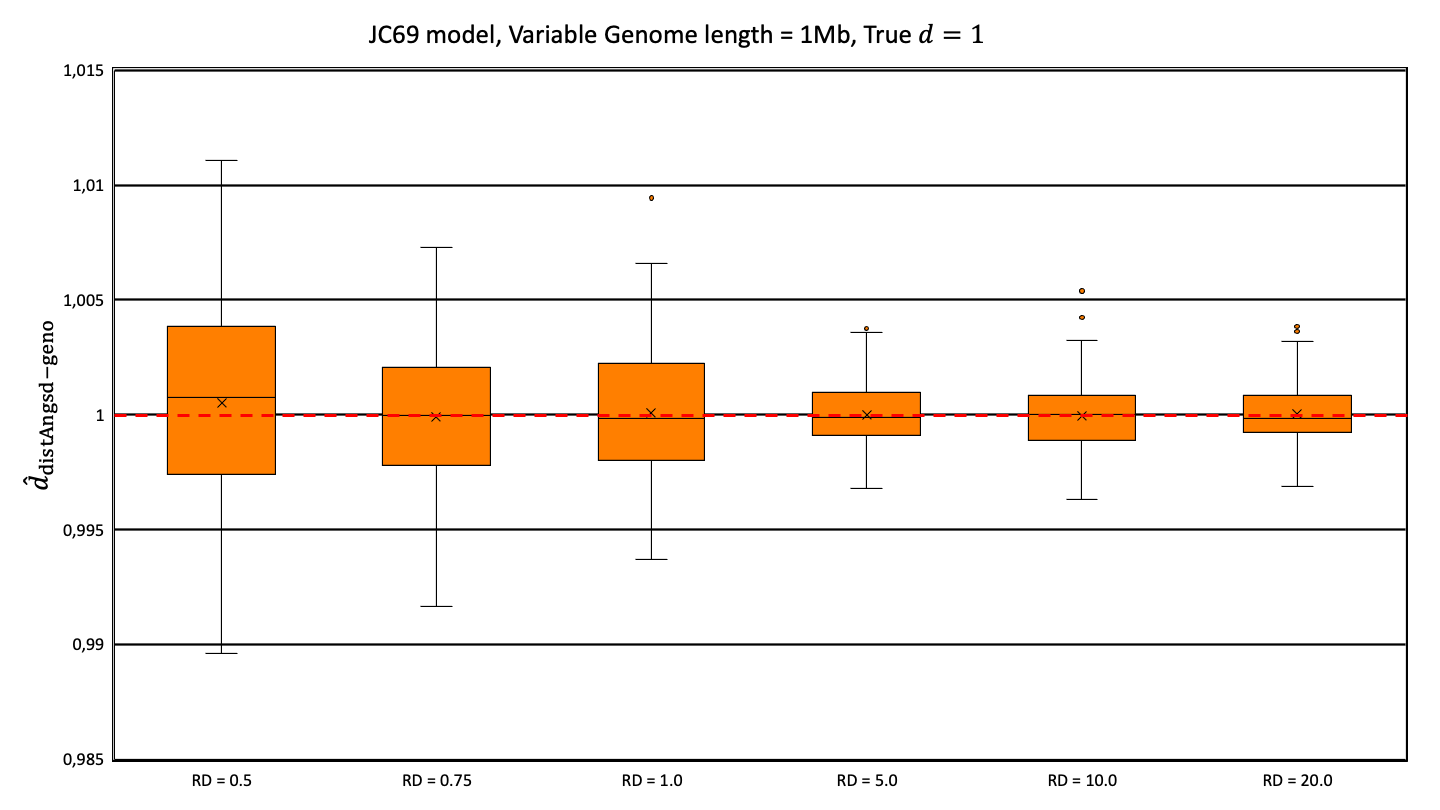
\includegraphics[width=\textwidth]{distAngsd-geno.png}
%          \caption{}
%          \label{fig:distAngsd-geno}
%      \end{subfigure}
%     \vspace{0.5cm}
%     \caption{JC69 model is simulated to compare the inference results of distAngsd-geno and ngsDist with different read depths, $20$, $10$, $5$, $1$, $0.75$ and $0.5$ and same true genetic distance $d=1$ (follows divergence tree as Fig. \ref{fig:basictree4inference}, with $t_1=0.4$ and $t_2 = 0.25$). Simulated genome lengths $1$Mb (a)(b) and $0.1$Mb (c)(d) are considered. With genotype likelihoods taken into account, The estimates of both ngsDist and distAngsd-geno are expected to fluctuated around some certain value as genome length varies. But ngsDist will not stay the same which is due to limited information of genotype likelihoods are used.}
%     \label{fig:}
% \end{figure*}

Our methods can also be extended to jointly estimate the fraction of invariable sites $p_{inv}$ and genetic distance $d$ quite accurately based on a pair of samples given the underlying GTR model is known. While other methods have quite larger biases in such joint inferences. This reflect the stability of distAngsd-geno and distAngsd-nuc (For details, see Table S1, FIG. S1,S2 and S3 in see Supplementary Information).
% \subsubsection{JC69 Model}

% \subsubsection{GTR Model}
% ???
\vspace{2mm}
\subsection{Inference based on Experimental Data}\label{subsec:ExpInfer}
From the appearances of the trees in FIG. \ref{fig:OakTree}, it seems that the distAngsd-geno tree can group the $83$ oak samples better compared with the other two trees, as it gives clearest boundaries between {\it Quercus berberidifolia}, {\it Quercus durata var. gabrielensis
} and {\it Quercus durata var. durata}. 

\begin{figure*}[h]
    \centering
    \begin{subfigure}[b]{0.95\textwidth}
    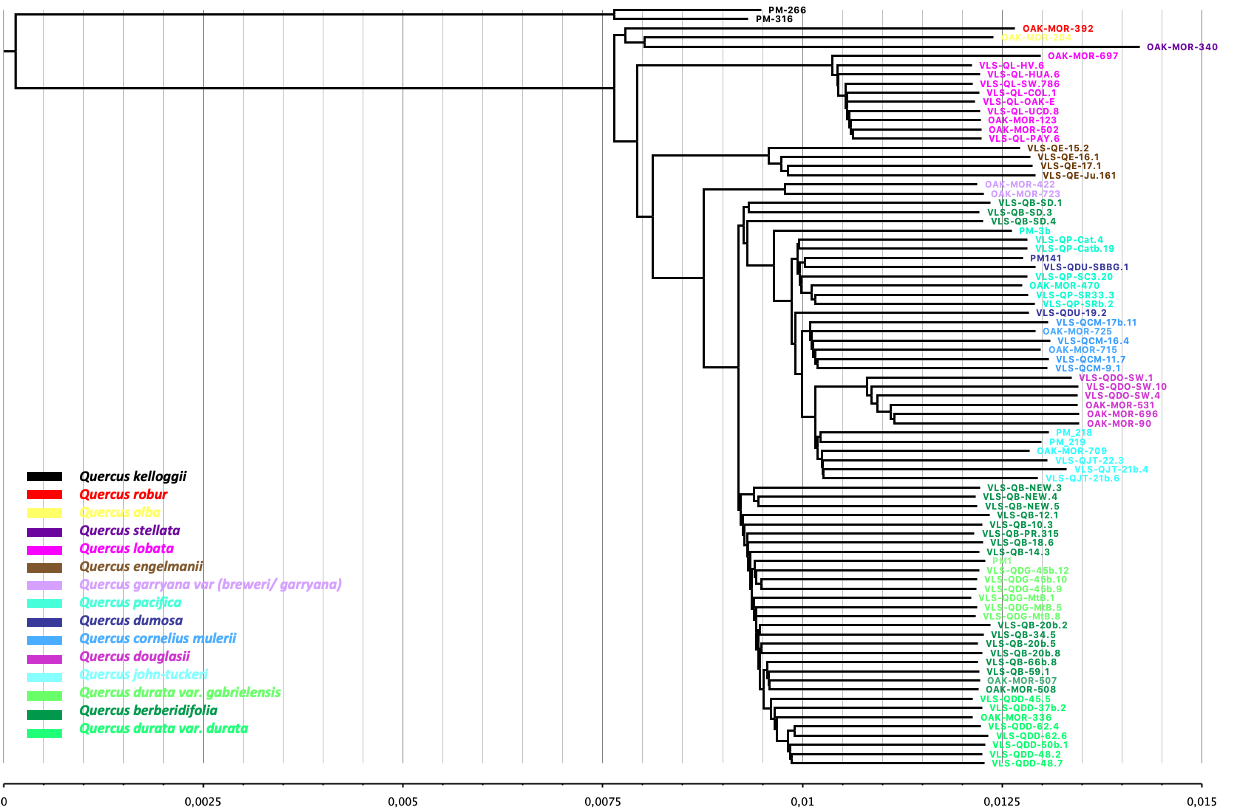
\includegraphics[width=\textwidth]{matrix_full_nofiltering.in_bionj.t1.png}
    \caption{distAngsd-geno inferred tree}
    \label{fig:distAngsd-genoOakTree}
    \end{subfigure}
    \begin{subfigure}[b]{0.95\textwidth}
    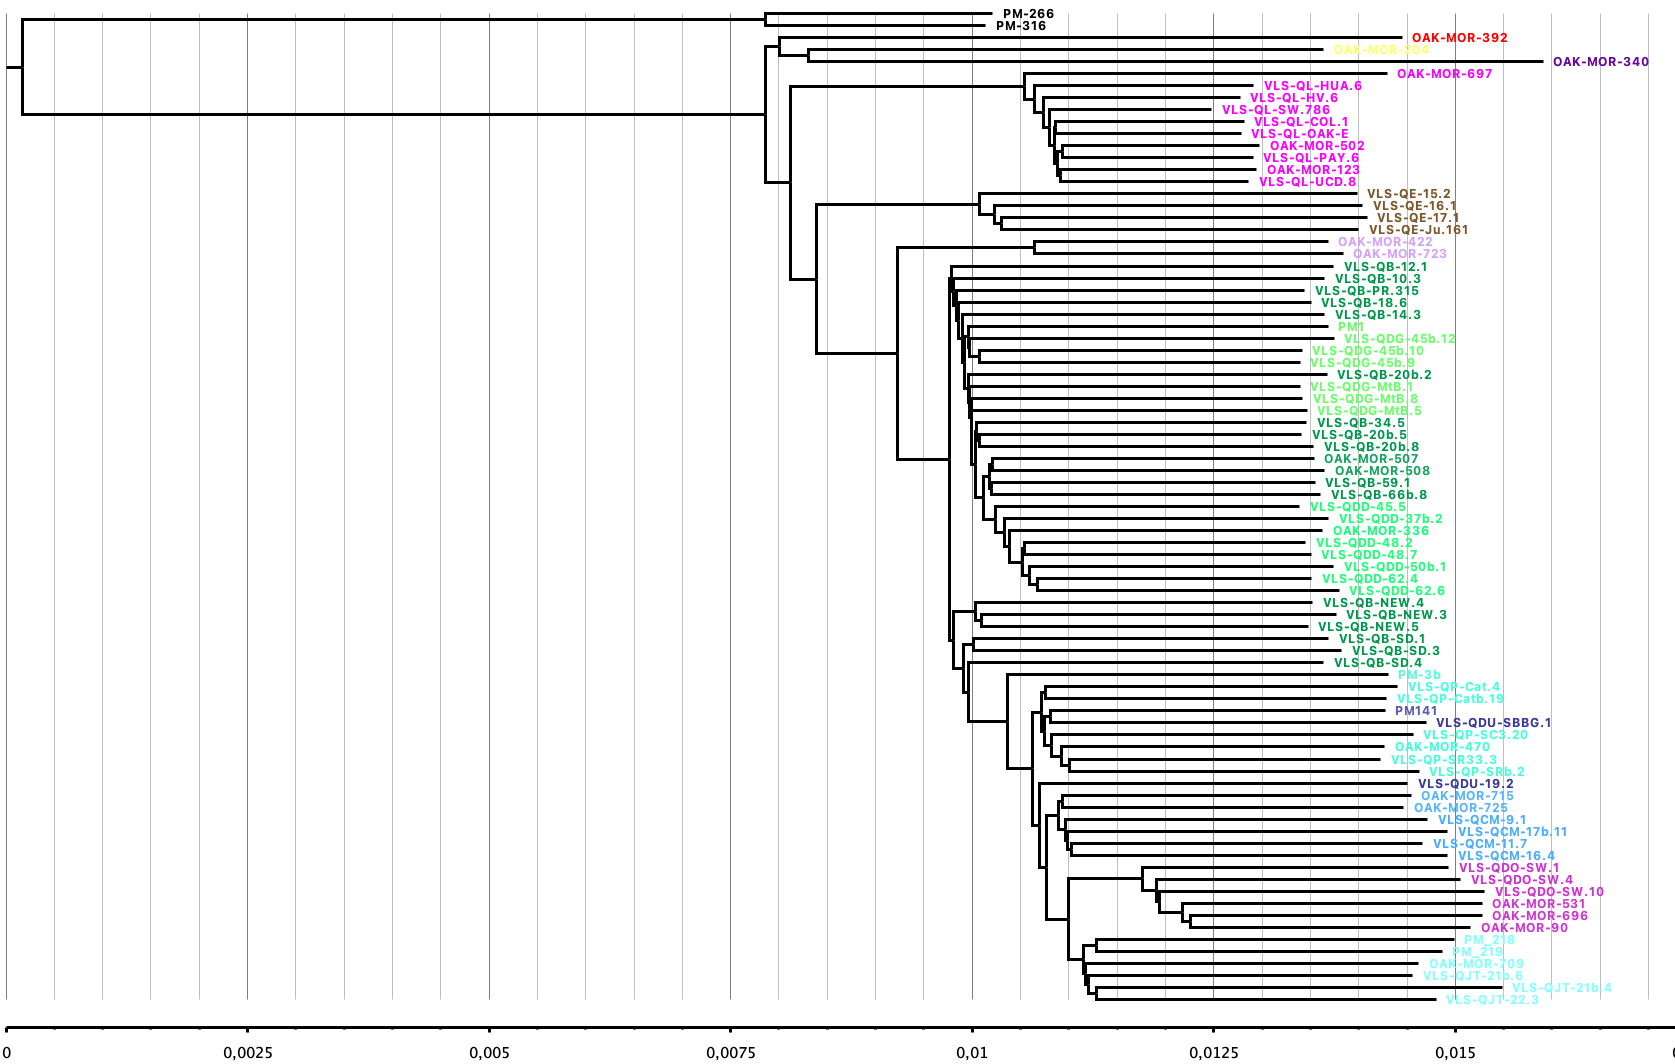
\includegraphics[width=\textwidth]{JCAmatrix_full_nofiltering_SEQ.in_bionj.t.png}
    \caption{ConsensusSEQ inferred tree}
    \label{fig:ConsensusSEQOakTree}
    \end{subfigure}
\end{figure*}
\begin{figure*}[ht]\ContinuedFloat
    \begin{subfigure}[b]{0.95\textwidth}
    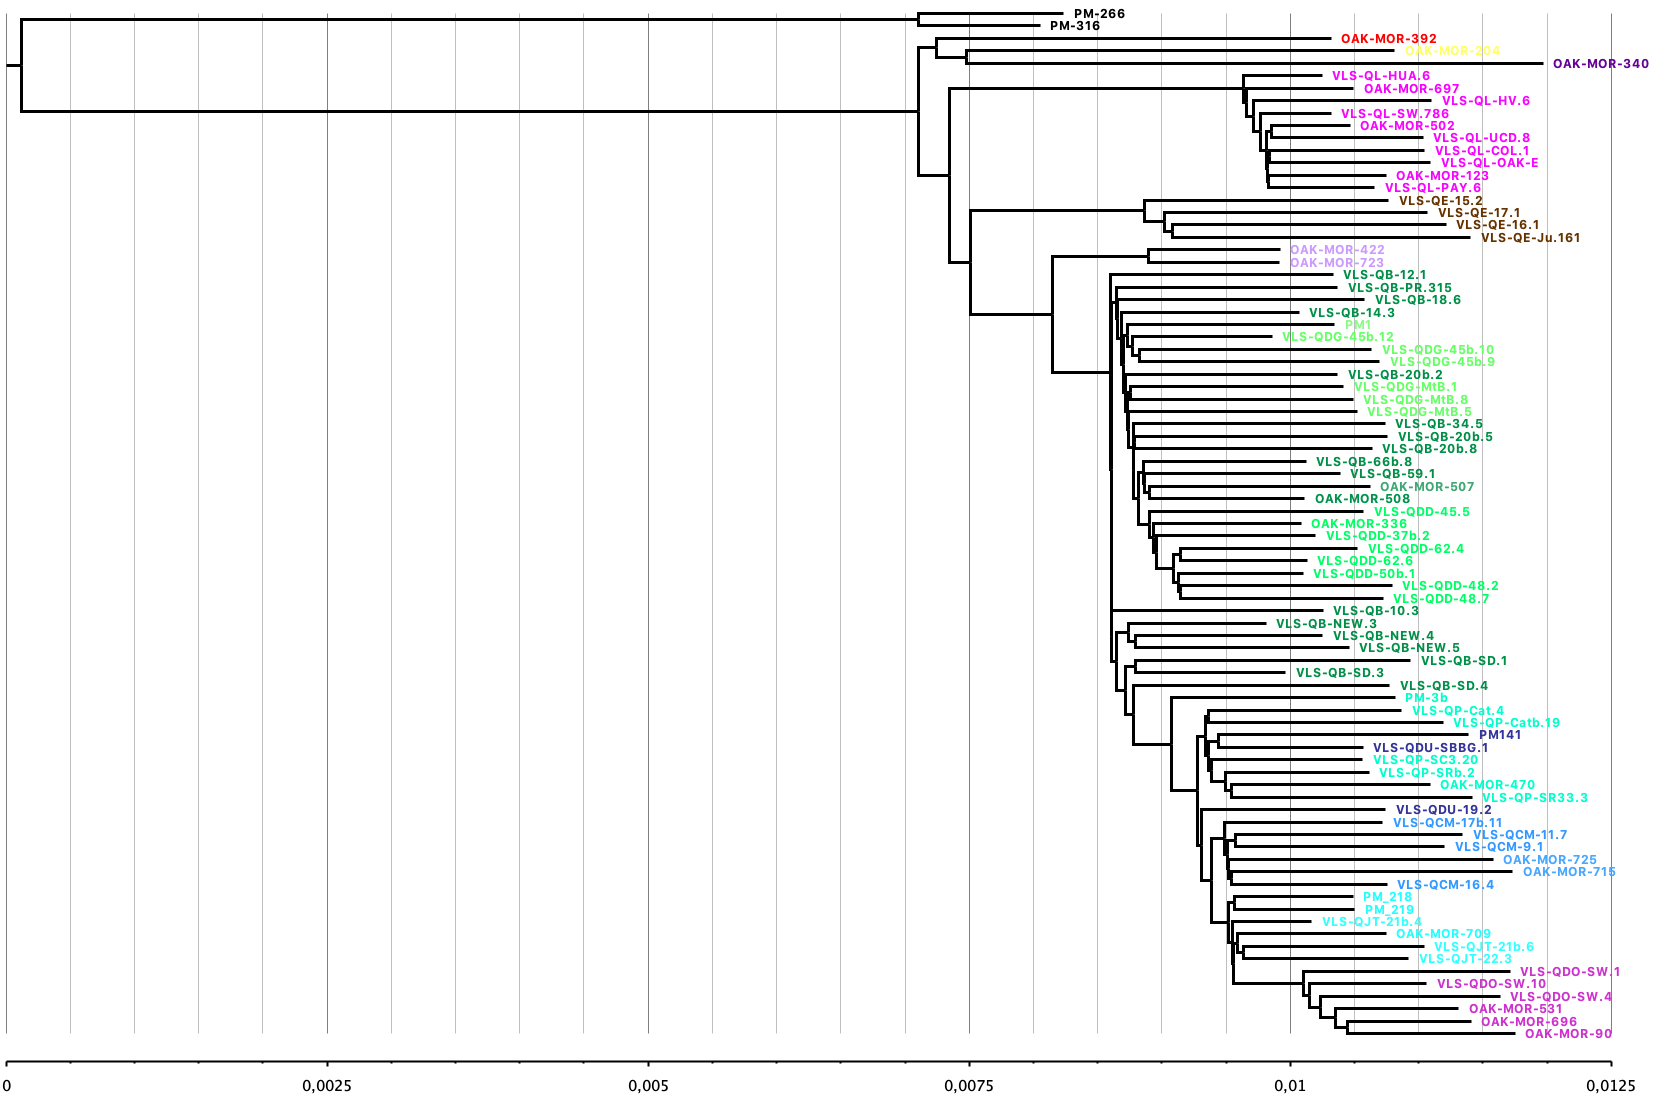
\includegraphics[width=\textwidth]{JCAmatrix_full_nofiltering.in_bionj.t.png}
    \caption{ConsensusGT inferred tree}
    \label{fig:ConsensusGTOakTree}
    \end{subfigure}
    \vspace{0.5cm}
    \caption{Neighbour-Joining Tree of $83$ oak inferred by (a) distAngsd-geno method (b) ConsensusSEQ method, and (c) ConsensusGT method. All these inferences are based on the JC69 model, the colors of the labeled names represent the species shown in the legend. The trees are all inferred by the full data rather than the downsampled data. All three trees are actually unrooted trees with roots placed between the known outgroup {\it Quercus kelloggii} and other Oak species.}
    \label{fig:OakTree}
\end{figure*}

All trees shown in FIG. \ref{fig:OakTree} are based on the full data which are the original $83$ oak samples with mean read depth $20.32$ (per sample) and lowest depth $10.34$. We further confirm this conclusion and test the inference capability of the new method by conducting downsampling to each sample. Based on the data with same level of mean depths (i.e., $10$, $5$, $1$, $0.75$, $0.5$, and $0.25$), neighbour-Joining trees inferred by different methods (distAngsd-geno method, ConsensusSEQ method and ConsensusGT method) are constructed.
And a compatibility measurement $m$ is developed (See in Supplementary Information) to check how well the inferred trees go with the prior species knowledge obtained from \cite{Fitz-Gibbon_Hipp_Pham_Manos_Sork:2017}. Table \ref{tab:DownsamplingExperimentalResults} shows the $m$ values of different trees with different mean depths based on different methods.

\begin{table*}[ht]
    \centering
    \begin{tabular}{|c|c|c|ccccccc|}
     \hline
     \multirow{4}{*}{Criterion $|\Omega_1\cap \Omega_2|=0$}& \multicolumn{2}{c|}{Downsampling depth} & full & $10$ & $5$ & $1$ & $0.75$ & $0.5$ & $0.25$\\
      \cline{2-10}
      & distAngsd-geno & \multirow{3}{*}{$m$} & 17 & 17 & 17 & 16 & 16 & 17 & 13 \\
      & ConsensusSEQ & & 17 & 17 & 17 & 16 & 16 & 16 & 13\\
      & ConsensusGT & & 16 & 16 & 16 & 16 & 16 & 16 & 12\\
      \hline
      \multirow{4}{*}{Criterion $|\Omega_1\cap \Omega_2|\leq 1$} &\multicolumn{2}{c|}{Downsampling depth} & full & $10$ & $5$ & $1$ & $0.75$ & $0.5$ & $0.25$\\
      \cline{2-10}
       & distAngsd-geno &\multirow{3}{*}{$m$} & 75 & 75 & 73 & 74 & 73 & 70 & 57 \\
      & ConsensusSEQ & & 74 & 75 & 76 & 72 & 70 & 66 & 58\\
      & ConsensusGT & & 75 & 75 & 74 & 74 & 70 & 67 & 56\\
    \hline
      \end{tabular}
    \caption{The compatibility measurement $m$ between the inferred pairwise distance trees and the prior species knowledge.The trees are inferred based on the original samples as well as the downsampled samples. The original 83 samples have mean read depth $20.32$ with lowest depth $10.34$, and each sample is downsampled to mean read depth $10$, $5$, $1$, $0.75$, $0.5$ and $0.25$.}
    \label{tab:DownsamplingExperimentalResults}
\end{table*}

The larger the compatibility measurement $m$ is, the better the tree go with the prior species knowledge. Table \ref{tab:DownsamplingExperimentalResults} can further validate that distAngsd-geno tree is better than both ConsensusSEQ and ConsensusGT trees when read depth is lower.

\vspace{2mm}
\section{Discussion}\label{sec:Discuss}
We have presented in the work two phylogeny inference methods, i.e., distAngsd-geno and distAngsd-nuc. With genotype likelihood taken into account, both methods can estimate the genetic distance between samples with high uncertainty, which are suitable for the area of ancient DNA where lower coverage is always the case. 

The key characteristic of the both methods is to decompose the likelihood optimization process into two parts, the EM algorithm to obtain the pseudo-observations of joint distribution of genotypes/sampled nucleotides per site between each pair of samples; the maximum likelihood scheme to infer genetic distance (and other related parameters) based on the pseudo-observations. EM algorithm part has nothing to do with the evolutionary model one adopted, thus can be conducted independently and in advance, and the downstream phylogeny inference will only depend on the inferred $10\times 10$ $\hat{\bf M}$ matrix or $4 \times 4$ $\hat{\bf N}$ matrix from the EM part. Thus, we believe our methods can serve as an interface to plug into any existing phylogeny inference software/method. The decomposition will also reduce the complexity of the overall log-likelihood function and reduce the computational costs to conduct the maximum likelihood algorithm.

At the cost of acquiring these advantages, we noted that the decomposition of likelihood optimization will introduce biases into the genetic distance estimators (See Supplementory Information S4). In most of the practical case, as the base calling error is around $0.2\%$, even the average read depth is $<1$, such biases are so small that will be absorbed into inference uncertainty. But when the base calling error is extremely high, the genome length is extremely short and the coverage is extremely low, these biases can be visible, and make the mean of the estimators different from the true value. Most of the pre-existing methods also suffer bias problem when dealing with samples of that bad quality, and our two methods actually create the smallest biases compared with them.

The distAngsd-geno present in this work are based on the prior knowledge that a diploid organism is concerned, it has the potential to extend to analyse any ploidy known organism at a cost of joint distribution matrix of genotypes $\mathbf{M}$ size increasing: For a $n$ ploid organism, the size of $\mathbf{M}$ will be ${n+3 \choose 3} \times {n+3 \choose 3}$. Unlike the distAngsd-geno, the distAngsd-nuc does not require any prior knowledge of ploidy level, and the size of joint distribution matrix of sampled nucleotides $\mathrm{N}$ will always stay $4 \times 4$. Without using any information of ploidy, distAngsd-nuc sometimes does not behave as good as distAngsd-geno does for the true variability which can be sorely explained by mutation and ploidy, but we believe it will work better once the variablity that can not explained by ploidy, e.g, contamination and change of ploidy along the genome. 

Joint estimation of genetic distance $d$ and fraction of invariable sites $p_{inv}$ are not expected from just a pair of samples. Mathematically, for some "symmetric" evolutionary model, it is even impossible to do so (e.g., JC69+I model, Supplementary Information S3.5.2). For some "asymmetric" GTR+I model, we have evidences that our methods can give better joint estimations compared with other methods, which will always have some visible biases. This in some sense shows the stability of our proposed distAngsd-geno and distAngsd-nuc methods.

The same idea of distAngsd-geno and distAngsd-nuc can be inplemented into a phylogeny software to to build up ML tree based on some more complex model (e.g., GTR+$\Gamma$+I model).
% Supplementary tables S1?S7 and figures S1?S11 are available  at Molecular Biology and Evolution
% online (http://www.mbe.oxfordjournals.org/).
\vspace{2mm}
\section{Acknowledgments}
We thank Prof. Victoria L. Sork and Dr. Sorel Fitz-Gibbon for kindly sharing the oak data with us.
We thank Prof. Rasmus Heller for advice of processing RAD sequences. Some of our function optimization codes were obtained from the corresponds between Prof. Ziheng Yang and Rasmus Nielsen, we thank Prof. Yang for kindly sharing these codes.
Funds?




\bibliographystyle{natbib}%%%%natbib.sty
\bibliography{refs}%%%refs.bib


\end{document}